%02 12 2014

\documentclass[journal]{IEEEtran}
% *** CITATION PACKAGES ***
\usepackage[sort&compress]{natbib}
%\usepackage{cite}






% *** GRAPHICS RELATED PACKAGES ***
%
%\ifCLASSINFOpdf
%  % \usepackage[pdftex]{graphicx}
%  % declare the path(s) where your graphic files are
%  % \graphicspath{{../pdf/}{../jpeg/}}
%  % and their extensions so you won't have to specify these with
%  % every instance of \includegraphics
%  % \DeclareGraphicsExtensions{.pdf,.jpeg,.png}
%\else
%  % or other class option (dvipsone, dvipdf, if not using dvips). graphicx
%  % will default to the driver specified in the system graphics.cfg if no
%  % driver is specified.
%  % \usepackage[dvips]{graphicx}
%  % declare the path(s) where your graphic files are
%  % \graphicspath{{../eps/}}
%  % and their extensions so you won't have to specify these with
%  % every instance of \includegraphics
%  % \DeclareGraphicsExtensions{.eps}
%\fi
\usepackage{graphicx}
\usepackage[caption=false,font=footnotesize]{subfig}
\usepackage{epstopdf}
\usepackage{multirow}
\usepackage{rotating}

\usepackage{color}



% *** MATH PACKAGES ***
\usepackage{breqn}


% correct bad hyphenation here
\hyphenation{op-tical net-works semi-conduc-tor}


\begin{document}
%
% paper title
% can use linebreaks \\ within to get better formatting as desired
% Do not put math or special symbols in the title.
%\title{LDA as Model of Physical Activity profiles in COPD patients}
\title{Identifying Physical Activity Profiles in COPD Patients Using Topic Models}
%
%
% author names and IEEE memberships
% note positions of commas and nonbreaking spaces ( ~ ) LaTeX will not break
% a structure at a ~ so this keeps an author's name from being broken across
% two lines.
% use \thanks{} to gain access to the first footnote area
% a separate \thanks must be used for each paragraph as LaTeX2e's \thanks
% was not built to handle multiple paragraphs
%

\author{Gabriele~Spina,
        Piero~Casale,
        J\"{o}rg~D.~Leuppi,        
        Paul~S.~Albert,         
        Emiel~F.~M.~Wouters,        
        Nidia~A.~Hernandes,
        Sally~J.~Singh,        
		Frank~W.~J.~M.~Smeenk,
        Arnoldus~J.~R.~van~Gestel,        
		Judith~Garcia-Aymerich,
		Richard~W.~Costello,		
		Ruth~Tal-Singer,
		Jennifer~Alison,
        Martijn~A.~Spruit,
        and~Albertus~C.~den~Brinker% <-this % stops a space
        
        
\thanks{G.~Spina is with the Department
of Electrical Engineering, Eindhoven University of Technology, and with Smart Sensing and Analysis Group, Philips Research, Eindhoven, The Netherlands,
e-mail: g.spina@tue.nl.}% <-this % stops a space
\thanks{P.~Casale is with the Department
of Electrical Engineering, Eindhoven University of Technology, The Netherlands.}
\thanks{J.~D.~Leuppi, is with Medical University Clinic, Cantonal Hospital Baselland, Liestal and Medical Faculty, University of Basel, Basel, Switzerland.}
\thanks{P.~S.~Albert is with School of Ageing and Chronic Disease, University Hospital Aintree, Liverpool, United Kingdom.}
\thanks{E.~F.~M.~Wouters is with the Department of Respiratory Medicine, Maastricht University Medical Center+ (MUMC+), Maastricht, The Netherlands.}
\thanks{N.~A.~Hernandes is with the Laboratory of Research in Respiratory Physiotherapy, Department of Physiotherapy, State University of Londrina (UEL), Londrina, Brazil.}
\thanks{S.~J.~Singh is with the NIHR EM CLAHRC - Centre for Exercise and Rehabilitation Science, University Hospitals, Leicester, United Kingdom.}
\thanks{F.~W.~J.~M.~Smeenk is with the Department of Respiratory Medicine, Catharina Hospital, Eindhoven, The Netherlands.}
\thanks{A.~J.~R.~van~Gestel is with the Pulmonary Division, University Hospital of Zurich, Zurich, Switzerland.}
\thanks{J.~Garcia-Aymerich is with the Centre for Research in Environmental Epidemiology (CREAL), Barcelona, Spain.}
\thanks{R.~W.~Costello is with the Department of Respiratory Medicine, Beaumont Hospital, Dublin, Ireland.}
\thanks{R.~Tal-Singer is with GlaxoSmithKline R\&D, King of Prussia, PA, United States of America.}
\thanks{J.~Alison is with Clinical and Rehabilitation Sciences, The University of Sydney, Sydney, NSW, Australia.}
\thanks{M.A.~Spruit is with Department of Research \& Education, Center of expertise for chronic organ failure (CIRO+), Horn, The Netherlands.}
\thanks{A.B.~den~Brinker is with Smart Sensing and Analysis Group, Philips Research, Eindhoven, The Netherlands.}% <-this % stops a space
}

%BEFORE
%\author{Michael~Shell,~\IEEEmembership{Member,~IEEE,}
%        John~Doe,~\IEEEmembership{Fellow,~OSA,}
%        and~Jane~Doe,~\IEEEmembership{Life~Fellow,~IEEE}% <-this % stops a space
%\thanks{M. Shell is with the Department
%of Electrical and Computer Engineering, Georgia Institute of Technology, Atlanta,
%GA, 30332 USA e-mail: (see http://www.michaelshell.org/contact.html).}% <-this % stops a space
%\thanks{J. Doe and J. Doe are with Anonymous University.}% <-this % stops a space
%\thanks{Manuscript received April 19, 2005; revised December 27, 2012.}}

% note the % following the last \IEEEmembership and also \thanks - 
% these prevent an unwanted space from occurring between the last author name
% and the end of the author line. i.e., if you had this:
% 
% \author{....lastname \thanks{...} \thanks{...} }
%                     ^------------^------------^----Do not want these spaces!
%
% a space would be appended to the last name and could cause every name on that
% line to be shifted left slightly. This is one of those "LaTeX things". For
% instance, "\textbf{A} \textbf{B}" will typeset as "A B" not "AB". To get
% "AB" then you have to do: "\textbf{A}\textbf{B}"
% \thanks is no different in this regard, so shield the last } of each \thanks
% that ends a line with a % and do not let a space in before the next \thanks.
% Spaces after \IEEEmembership other than the last one are OK (and needed) as
% you are supposed to have spaces between the names. For what it is worth,
% this is a minor point as most people would not even notice if the said evil
% space somehow managed to creep in.



% The paper headers
\markboth{Journal of \LaTeX\ Class Files,~Vol.~11, No.~4, December~2012}%
{Shell \MakeLowercase{\textit{et al.}}: Bare Demo of IEEEtran.cls for Journals}
% The only time the second header will appear is for the odd numbered pages
% after the title page when using the twoside option.
% 
% *** Note that you probably will NOT want to include the author's ***
% *** name in the headers of peer review papers.                   ***
% You can use \ifCLASSOPTIONpeerreview for conditional compilation here if
% you desire.




% If you want to put a publisher's ID mark on the page you can do it like
% this:
%\IEEEpubid{0000--0000/00\$00.00~\copyright~2012 IEEE}
% Remember, if you use this you must call \IEEEpubidadjcol in the second
% column for its text to clear the IEEEpubid mark.



% use for special paper notices
%\IEEEspecialpapernotice{(Invited Paper)}




% make the title area
\maketitle

% As a general rule, do not put math, special symbols or citations
% in the abstract or keywords.
\begin{abstract}
With the growing amount of physical activity (PA) measures available, the need for methods and algorithms to automatically analyze and interpret unannotated data increases. In this paper PA is seen as a combination of multimodal constructs that can co-occur in different way and proportion during the day. The design of a methodology able to integrate and analyze them is discussed and its operation is illustrated by applying it to a data set comprising data from 997 COPD patients and 66 healthy subjects.
The method encompasses different stages. The first stage is a completely automated method of labeling low-level multimodal PA measures. The information contained in the PA labels are further structured using topic modelling techniques, a machine learning method from the text processing community. The topic modelling discovers the main themes that pervade a large set of data, in this case it discovers PA routines that are active in the assessed days of the subjects under study. Applying the designed algorithm to our data provides new learnings and insights. As expected, the algorithm discovers that the PA routines for COPD patients and healthy subjects are substantially different regarding their composition and moments in time in which transitions occur. 
Furthermore, it shows certain consistent trends relating to disease severity as measured by standard clinical practice.


%Inspired by machine learning methods from the text processing community, the daily stream of data coming from the Sensewear device is converted into a series of documents consisting of sets of discrete PA labels. Learning of the labels is performed in a fully unsupervised fashion by mean of clustering techniques. The sets of documents are then mined for common topics, i.e. activity patterns or routines that show the same probability distribution across the labels. Latent Dirichlet Allocation (LDA) is used to both extract the routines from the set of labels and to infer the day of the subjects in order to find the daily routine-activation probabilities that characterize patients and healthy subjects. Results show not only that the routines found are substantially different for COPD patients and healthy subjects, but also that the transitions between routines occur at different time. The discovered activity pattern and differences could be used, from an application point of view, to guide the patients in their rehabilitation program.
\end{abstract} 



% Note that keywords are not normally used for peerreview papers.
\begin{IEEEkeywords}
Activity routine, COPD, topic models.
\end{IEEEkeywords}






% For peer review papers, you can put extra information on the cover
% page as needed:
% \ifCLASSOPTIONpeerreview
% \begin{center} \bfseries EDICS Category: 3-BBND \end{center}
% \fi
%
% For peerreview papers, this IEEEtran command inserts a page break and
% creates the second title. It will be ignored for other modes.
\IEEEpeerreviewmaketitle


\newpage
\section{Introduction}
%02 12 2014

\IEEEPARstart{T}{he} prevalence of chronic diseases in general is rising due to an aging population as well as to  environmental and lifestyle changes.  This is particularly true for respiratory diseases such as Chronic Obstructive Pulmonary Disease (COPD), which is a progressive and irreversible disease that results in airflow limitation and significant extra pulmonary effects which limit physical activities~\cite{Seymour_2009, Verboom_2011}. 
Physical activity (PA), defined as any bodily  movement produced by skeletal muscles that requires energy expenditure~\cite{Caspersen_1985}, is known to be a relevant indicator of COPD patients health state. Research on  physical activity levels of COPD patients has consistently shown that COPD patients have lower physical activity levels than their healthy peers~\cite{Vorrink_2011}. Moreover, reduced levels of PA have been found to be related to an increased risk of hospital admission and mortality among COPD patients~\cite{Garcia_2006, Pitta_2006, Waschki_2011}. Outcome variables related to this type of analysis mainly focused on amount and volume parameters, such as
number of steps, volume of physical activity as expressed by total 
number of counts, and total energy expenditure. Although these are important health markers of patients suffering from COPD, interventions thus far have failed to demonstrate important increases in physical activities in patients with COPD. A better insight into daily PAs of patients with COPD needs to be achieved in order to assist in targeted therapeutic strategies and personalized coaching programs. In order to quantify PA it is not only necessary to measure a set of multidimensional parameters as the one mentioned above, but also their co-occurrence and temporal pattern. Moreover, when analyzing PA, physiological responses such as heart rate, temperature or galvanic skin response should be considered complementary constructs that needs to be harmoniously integrated with PA measures into meaningful descriptors.
With recent improvements in wearable sensor technologies it becomes easier in daily life to acquire massive amounts of different sensors data. At the same time, however, it is difficult to combine and extrapolate meaningful information in absence of any supervision or annotation.
A PA descriptor could be seen as a composite of multiple low-level PA measures, including their physiological responses, that can co-occur in a different way and proportion i.e., PA routines. Routines could also occur at different time and in different proportion across the day for different patients or subgroups of patients characterizing their activity behaviour. The reader might think about PA measures and physiological responses as the letters composing the words that describe PAs. The co-occurrency of these words creates groups of PA constructs describing the main topics that pervade the day of a patient. 
This work aims at studying low-level multimodal sensor data in order to find unknown and characteristic PA structures, able to quantify difference among COPD and healthy subjects (matching for gender age and BMI) and within COPD severity classes. This is particularly difficult in this patient population
since it is known that COPD patients maintain a constant
inactive behaviour during the day that makes standard activity
recognition tools not suitable for the purpose.\\
%In particular, this paper provides the following contributions:
%\begin{enumerate}
%\item We proposes an automatic data mining method based on multimodal physical activity measures able to quantify differences in physical activity routines between 66 COPD patients and 66 healthy control subjects.
%\item We proposes an automatic data mining method based on topic modelling, able to discover activity routines as a probabilitstic combination of multimodal physcal activity measures.
%\item We identify differences in the physical activity routines discovered between 66 COPD patients and 66 healthy control subjects.
%\item We propose LDA as Model of Physical Activity profiles in COPD patients
%\item We identify how activity patterns are distributed across time, what are the typical active periods during daily life of patients living at home in a group of 977 COPD patients and we individuate differences between COPD severity classes.
%\item We propose daily routines as a better identifier of active or sedentary life style. 
%\end{enumerate}
In particular, this paper provides the following contributions: (1) we propose a methodology to create a vocabulary of meaningful words from a set of mutimodal PA measures without the need of any supervision or parameter tuning, (2) we discover PA routines that pervade daily life of COPD patients. Finally, (3) we infer the underlying PA routine structure of numerous patients data quantifying differences between COPD patientsa and healthy subjects and among COPD patients. In particular, for each assessed day we infer which is the distribution over the routines in day segments of 30 minutes, describing in such a way the temporal regularities of the multidimodal PA measures.


%PA should be regarded as a multi-dimensional construct~\cite{Bussmann_2013}, which means that it should be described by relevant constructs and parameters other than the total amount of PA only. 

%Over the last few decades, the methods used to objectively assess
%a person's behavior in terms of body postures (e.g., sitting, standing), body movements(e.g., walking, cycling),and/or daily activities (e.g., sports, gardening) in a daily life setting have improved considerably. Devices have become smaller, power consumption requirements have decreased, data storage capacity has increased, and innovative, integrated sensors have been developed. 

%These developments and outcome variables have contributed to a better understanding of daily behavior and a more accepted role of it in research and clinical practice.




%For comparison the average values of METs and the standard error (SE) during the days for COPD patients and heathy subjects could be observed in Fig.\ref{fig:2}. 
%Previous analysis failed because taking only the average as you can see from Fig.~\ref{fig:2} after 1 hour from the waking up moment the standard error of the mean increases again.



%Moreover, patients are not able to accurately self-report their physical
%activities~\cite{Pitta_2007}. The method, then, needs to be unsupervised without the needs of using annotations.


%\newpage
\section{Related works}

The automatic monitoring and analysis of chronic diseases has always been central in research on wearable sensors. In particular, the continuous monitoring of COPD patients has gained considerable interests in the recent years. Liao et al.~\cite{Liao_2014} provided a review focused on describing current wearable technologies for measuring the physical activity level of COPD patients. Dimensions such as reliability, validity, advantages and limitations are discussed. Of particular interest is the work of Patel et al.~\cite{Patel_2007} where a comparative study of machine learning techniques is presented in order to track changes in physiological responses of COPD patients with respect to their physical activity level. They used motion data to monitor activities in conjunction with heart-rate and respiration rate to capture the physiological responses of the patients while performing a set of activities. Beattie et al.~\cite{Beattie_2014} considered how the early detection of disease exacerbation can lead to earlier provision of intervention advice. These authors focus on important parameters for patients self-management such as autonomy, methods of data transmission and levels of intrusiveness and propose guidelines for the development of a context-aware system aimed at overcoming current limitations in the perspective of a user-friendly system for the patients. More advanced self-management platforms have been recently proposed. For example, Bellos et al.~\cite{Bellos_2014} propose an integrated platform aiming at the effective management and real-time assessment of the health status of COPD patients.
A combination of machine-learning techniques was able to provide real-time categorizations of COPD episodes  and estimate the severity of pathological situations in different levels, triggering an alerting mechanism for the patient and the clinical supervisor. 
%\textbf{Add here the main limitation of these works.Add here the main limitation of these works.Add here the main limitation of these works. Add here the main limitation of these works. Add here the main limitation of these works.}

Topic models represent a class of algorithms able to discover hidden thematic structure in collections of documents. Due to their pattern discovery nature, they have been widely explored in the wearable sensor and activity recognition community. 
Huyn at al.~\cite{Huynh_2008} showed that the activity patterns discovered using topic modelling approaches correspond to high-level users' behavior. Authors used activity patterns based on a learned vocabulary of meaningful events such as walking, using the phone, discussing at whiteboard, etc. These authors also addressed the point of avoiding supervised learning approaches using unsupervised methods for building the vocabulary using a clustering approach. Qualitative results show that high-level structure of the data as well as activity transitions, novelties and anomalies can be discovered using their approach.
Seiter et al.~\cite{Seiter_2014} investigated unsupervised activity discovery approaches using three topic model approaches. Authors analyzed three public datasets with different properties affecting the discovery such as primitive rate, activity composite specificity, primitive sequence similarity, and composite-instance ratio. They compared the activity composite discovery performance against the performance of a k-means clustering algorithms providing guidelines for optimal parameter selection. Results indicated that LDA shows higher robustness against noise compared to k-means and other topic modelling approaches. 
%\textbf{Look for one more supporting the hypothesis of the paper and Add here the motivation why those approaches are not completely suitable for the problem at hand.}


%\section{Topic models}
%02 12 2014

Topic models are algorithms for discovering the main themes that pervade a large and otherwise unstructured collection of documents.
The idea behind probabilistic modelling is to treat data as observations arising from a generative probabilistic process that includes hidden variables. This hidden layer of organization, whereby observations are structured, is what we want to find in the data. 
In the field of text mining the hidden variables reflect the thematic structure (that we do not have access to) of a collection of text documents composed by words. In our case the hidden variables represent the unknown activity routines that a subject performs during a day.
In a text document what is observed are the words. We, instead, observe a set of variables that are related to the activities of daily living performed by a subject during several days.

%Other possible version
%In the field of text mining the hidden variables reflect the thematic structure (that we do not have access to) of a collection of text documents composed by words. In our case the hidden variables represent the unknown activity routines that link together activity primitives like walking, sitting standing that a subject performs during a day. 
%In a text document what is observed are the words. Observing activity primitives in patients is tricky since the subjects should be asked to annotate what he or she does during the day or activity primitives should be recognized from measurable variables like limbs accelerations. This introduce errors that could propagate in the routine discovery.
%We, instead, observe a set of variables that are related to the activities of daily living performed by a subject during several days.

Following this preamble the intuition behind the use of the Latent Dirichelet Allocation (LDA) in activity routine discovery is that each day is a mixture of thematically coherent activities (routines) as a text document is a mixture of thematically coherent terms (topics). %exhibits
The graphical model for LDA is provided in Fig.~\ref{fig:LDA_model}.

%%%%%%%%%%%%%%%%%%%%%%%%%%%%	FIGURE TOPICMODEL		%%%%%%%%%%%%%%%%%%%%%%%%%%%%
\begin{figure}[ht]
\centering
    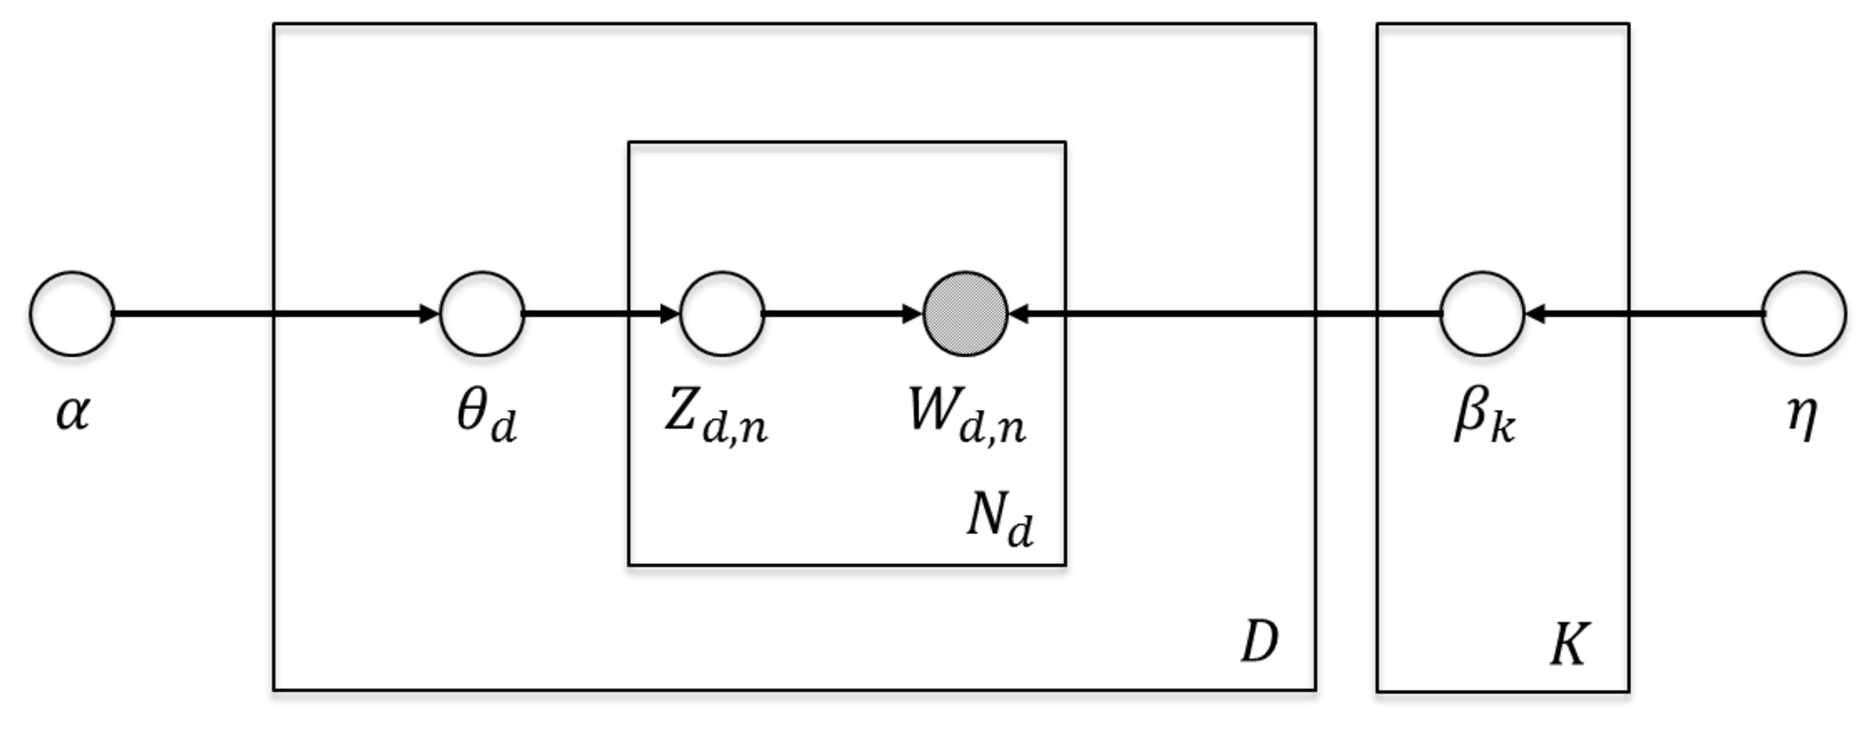
\includegraphics[width=.40\textwidth]{figure/eps/LDA_model.eps}
  \caption{Graphical model for LDA.Observations: words-documents.
Hidden structure: topjc structure, topics per document topic distributio, and the per document per word topic assignments.}\label{fig:LDA_model}
\end{figure}
%%%%%%%%%%%%%%%%%%%%%%%%%%%%%%%%%%%%%%%%%%%%%%%%%%%%%%%%%%%%%%%%%%%%%%%%%%%

All the documents ($d_{1:D}$) in the collection share the same set of topics ($\beta_{1:K}$) that are defined as Dirichelet distributions over the words ($w$) of a fixed vocabulary. Each document exhibits topics in different proportion indicated as $\theta_{1:D}$, i.e. each document has a different distribution over the topics that also follow a Dirichelet distribution. The distribution of the words in a topic and of the topics in a document depend only on the topic hyper-parameters $\eta$ and $\alpha$ that control the mean shape and sparsity of the distributions. In such a model the $N$ words ($w_{d,n_{1:N}}$) that compose the $d$ document are the only random variables observed and depend on the per word topic assignment ($Z_{d,n}$) and all the $\beta_{k}$.
%
%i.e. they are composed by words that belong, with a certain probability distribution, to different thematic areas. 
%
%The idea is to express the intuition as a generative probabilistic process:
%first we are gonna posit that there are some number of topics that we re going to define that live outside the document collecion.
%For example here there are 4 topics listed and each topic is a distribution over a fixed vocabulary. There is a fixed vocabulary and each
%topic is a distribution over that fixed vocabulary. Different topics have different words with different probabilities.
%
%The generative process for each document works like this:
%We re going to choose a distribution over topics. 
%We are gonna draw this distribution from a Dirichelet distribution.
%
%Each document is a random mixture of corpus-wide topics.
%Each word is drawn from on of those topics.
The generative process defines a joint probability distribution (\ref{eq:jointdistr}) over both the observed and hidden random variables. 

\begin{dmath}
  p(\beta_{1:K},\theta_{1:D},z_{1:D},w_{1:D}) = \prod_{k=1}^{K} p(\beta_{k}|\eta) \prod_{d=1}^{D} p(\theta_{d}|\alpha) \prod_{n=1}^{N} p(z_{d,n}|\theta_{d}) p(w_{d,n}|z_{d,n},\beta_{1:K}).
  \label{eq:jointdistr}
\end{dmath}

Reversing the generative process, it is possible to calculate the hidden structure that likely generated the observed collection. More formally the joint probability distribution is used to compute the conditional distribution~(\ref{eq:conddistr}) of the hidden variables given the observed variables. 
\begin{dmath}
  p(\beta_{1:K},\theta_{1:D},z_{1:D}|w_{1:D}) =   \frac{p(\beta_{1:K},\theta_{1:D},z_{1:D},w_{1:D})}{p(w_{1:D}}.
  \label{eq:conddistr}
\end{dmath}
This conditional distribution is also called the posterior distribution that is intractable to compute. Topic modelling algorithms form an approximation of~(\ref{eq:conddistr}) by adapting an alternative distribution over the latent topic structure to be close to the true posterior. In particular, for this analysis, we use variational inference that posits a parameterized family of distributions over the hidden structure and then find the member of that family that is closest to the posterior according to \emph{Kullback-Leibler} divergence.
%It is implicitly assumed that the order of words does not matter. %Because I choosing those coins independtly of each other.
%If there is a documents which words are shuffled we might still understand the meaning looking at the different type of words that occur in the document.
In our analysis the goal is to infer the underlying topic structure of numerous patients data.
Given the documents first of all we look for what are the topics (i.e. distributions of terms of the vocabulary) that generated them under these assumptions, secondly for each document we infer which is the distribution over topics associated with that document. We compare results from COPD patients with healthy subjects and within COPD classes.







%LDA falls precisely into this framework.
%The observed variables are the words of the documents; the hidden variables are the topic structure; and the generative process is as described here. The computational problem of inferring the hidden topic structure from the documents is the problem of computing the posterior distribution, the conditional distribution of the hidden variables given the documents.
%We can describe LDA more formally with the following notation. The topics
%are b1:K, where each bk is a distribution over the vocabulary. The topic proportions for the dth document are qd, where qd,k is the topic proportion for topic k in document d (the cartoon histogram in Figure 1). The topic assignments for the dth document are zd, where zd,n is the topic assignment for the nth word in document d (the colored coin in Figure 1). Finally, the observed words for document d are wd, where wd,n is the nth word in document d, which is an element from the fixed vocabulary.

\section{Unsupervised Routine discovery}
%02 12 2014
Topic models are algorithms for discovering the main themes that pervade a large and otherwise unstructured collection of documents. Data are treated as observations arising from a generative probabilistic process in which hidden variables reflect the thematic structure of a collection of documents. The intuition behind the use of the Latent Dirichelet Allocation (LDA) to discover PA routines is that each day is a mixture of thematically coherent PA measures as a text document is a mixture of thematically coherent terms. The graphical model for LDA is provided in Fig.~\ref{fig:LDA_model}.
%%%%%%%%%%%%%%%%%%%%%%%%%%%%	FIGURE TOPICMODEL		%%%%%%%%%%%%%%%%%%%%%%%%%%%%
\begin{figure}[ht]
\centering
    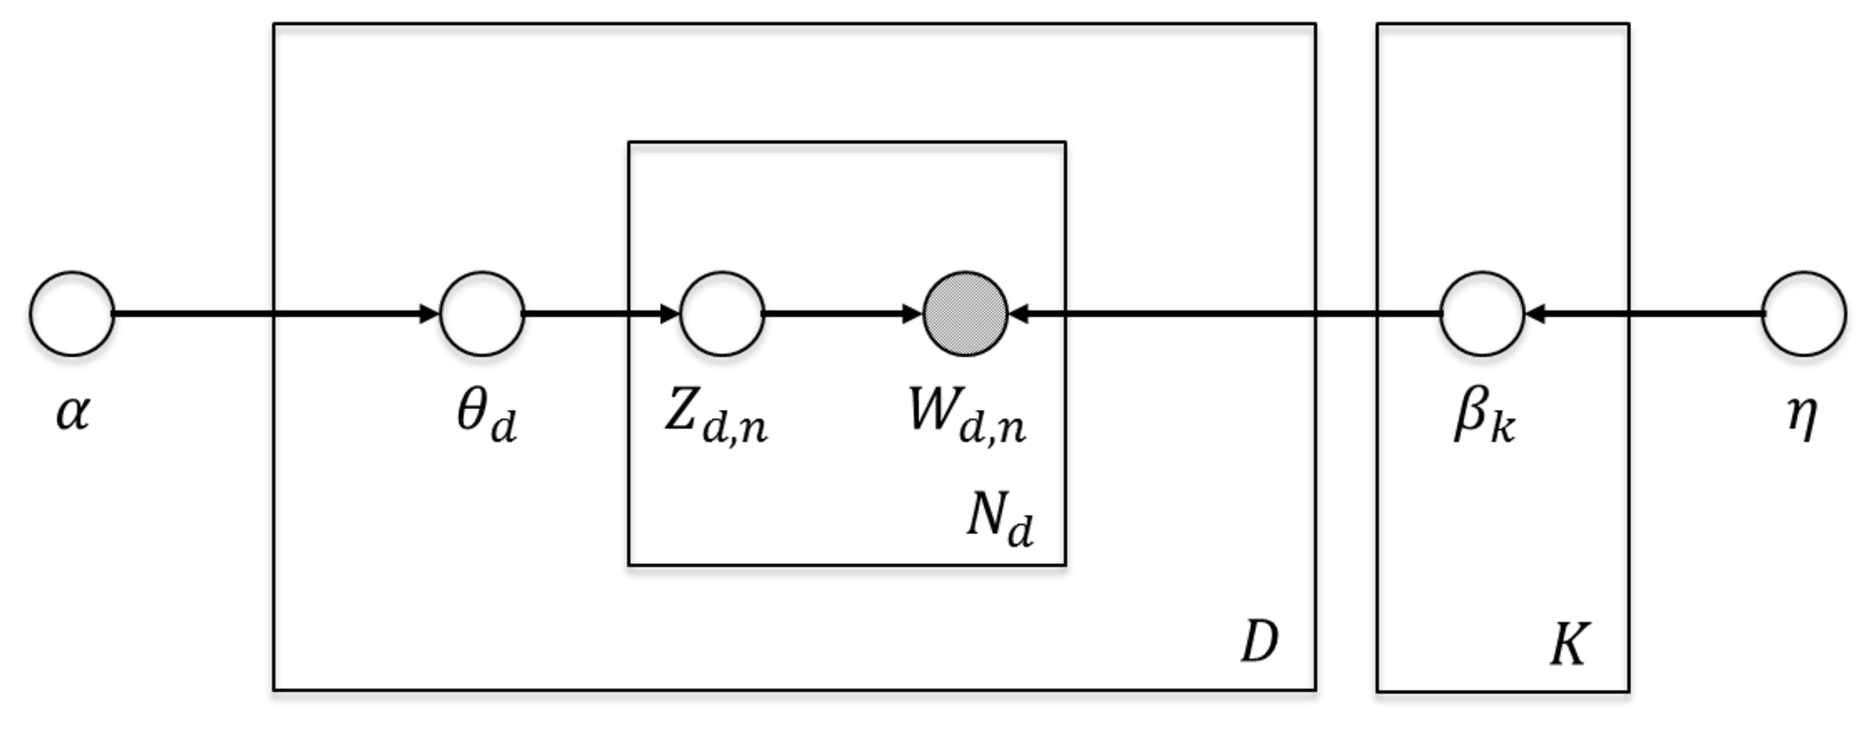
\includegraphics[width=.40\textwidth]{figure/eps/LDA_model.eps}
  \caption{Graphical model for LDA. Each node is a random variables, edges denote possible dependences. The only observed variables are the words (shaded).}\label{fig:LDA_model}
\end{figure}
%%%%%%%%%%%%%%%%%%%%%%%%%%%%%%%%%%%%%%%%%%%%%%%%%%%%%%%%%%%%%%%%%%%%%%%%%%%
All the assessed days (also called documents $d_{1:D}$) share the same set of daily routines (also called topics $\beta_{1:K}$) that are defined as Dirichelet distributions over the observed set of PA descriptors (also called words $W$ of a fixed vocabulary). Observing activities in patients is a difficult task since it is time-intensive and intrusive. At the same time patients are not able to accurately self-report their physical activities~\cite{Pitta_2007} and the training of a classifier requires annotations that in a daily life scenario are difficult to obtain. In order to make the methodology fully unsupervised we assume that the observed words (input of the model) are composed by multimodal PA measures coming from a body area sensor network.
Each assessed day exhibits PA daily routines in different proportion indicated as $\theta_{1:D}$, i.e. each day has a different distribution over the routines that also follow a Dirichelet distribution. The distribution of the words in a routine and the distribution of the routine in a document depend only on the topic hyper-parameters $\eta$ and $\alpha$ that control the mean shape and sparsity of the distributions. In such a model the $N$ words ($W_{d,n_{1:N}}$) that compose the $D$ documents are the only random variables observed and depend on the per word topic assignment ($Z_{d,n}$) and all the $\beta_{k}$.
The daily routines then are composed indirectly by low-level PA measures that belong, with a certain probability distribution, to different thematic areas. Different routines will have different PA measures with different probabilities. The generative process of the model defines a joint probability distribution over both the observed and hidden random variables, according to:
\begin{dmath*}
  p(\beta_{1:K},\theta_{1:D},Z_{1:D},W_{1:D}) = \prod_{k=1}^{K} p(\beta_{k}|\eta) \prod_{d=1}^{D} p(\theta_{d}|\alpha) \prod_{n=1}^{N} p(Z_{d,n}|\theta_{d}) p(W_{d,n}|Z_{d,n},\beta_{1:K}).
\nonumber\end{dmath*}
Reversing the generative process, it is possible to calculate the hidden structure that likely generated the observed collection of document. More formally the joint probability distribution is used to compute the conditional distribution of the hidden variables given the observed variables by: 
\begin{dmath}
  p(\beta_{1:K},\theta_{1:D},Z_{1:D}|W_{1:D}) =   \frac{p(\beta_{1:K},\theta_{1:D},Z_{1:D},W_{1:D})}{p(W_{1:D})}.
  \label{eq:conddistr}
\end{dmath}
This conditional distribution is also called the posterior distribution and it is intractable to compute. Topic modelling algorithms compute an approximation of~(\ref{eq:conddistr}) by finding a distribution over the latent topic structure to be close to the true posterior. In particular, for this analysis, we use variational inference that posits a parameterized family of distributions over the hidden structure and then finds the member of that family that is closest to the posterior according to \emph{Kullback-Leibler} divergence.

%put in the claims
%In the implementation described in the follwing paragraph we propose a methodology to create a vocabulary of meaningful words from a set of mutimodal PA measures, we discover PA routines that pervade daily life of COPD patients. Finally, we infer the underlying topic structure of numerous patients data. In particular, for each assessed day we infer which is the distribution over the routines found and we describe the temporal regularities of the multidimensional constructs and parameter of PA.




%LDA falls precisely into this framework.
%The observed variables are the words of the documents; the hidden variables are the topic structure; and the generative process is as described here. The computational problem of inferring the hidden topic structure from the documents is the problem of computing the posterior distribution, the conditional distribution of the hidden variables given the documents.
%We can describe LDA more formally with the following notation. The topics
%are b1:K, where each bk is a distribution over the vocabulary. The topic proportions for the dth document are qd, where qd,k is the topic proportion for topic k in document d (the cartoon histogram in Figure 1). The topic assignments for the dth document are zd, where zd,n is the topic assignment for the nth word in document d (the colored coin in Figure 1). Finally, the observed words for document d are wd, where wd,n is the nth word in document d, which is an element from the fixed vocabulary.


%\newpage
\section{Implementation and evaluation}
%03 12 2014
\subsection{Dataset}
Physical activity of a subject was assessed during daily life by mean of the SenseWear Armband and SenseWear Mini Armband activity monitors. 
These devices combine an accelerometer with different physiological sensors (a heat flux sensor, a galvanic skin response sensor, 
a skin temperature sensor, and a near-body ambient temperature sensor).  Together with demographic characteristics, such as gender, 
age, height and weight, energy expenditure (EE) and metabolic equivalent of task (MET) were estimated using proprietary algorithms 
developed by the manufacturer. Moreover, information about the sleeping status of a subject (0=awake, 1=sleeping) is also provided. 
The SenseWear Armband has been shown to be valid both in field~\cite{Colbert_2011,Mackey_2011} and in laboratory 
studies~\cite{Furlanetto_2010,Hill_2010,Cavalheri_2011}.
\par Data from 1001 COPD patients (65\% men; age, 67 years; $FEV_{1}$, 49\% predicted; BMI, 25.8) were recorded across 10 different countries. Subjects wore the sensor both during day time and night time so that continuous, non-scripted activities were recorded in a natural environment with 1 minute resolution. 
A minimum of 4 days (2 weekdays + Saturday + Sunday) was considered acceptable to include a patient in the analysis~\cite{Watz_2009}, with the device 
being used for at least 22 hours per day. 
%Since data presents intrinsic variability due to different
%awakening and sleeping times of the subjects we tried
%to minimize this synchronizing the days according to the
%morning awakening points, considered as the time instant
%after the longest period of sleep. Data before the awakening
%point were discarded from the analysis.
In order to minimize the intrinsic variability of data 
%that is due to different subjects' awake and sleep periods. Data prior to the awakening point was discarded from the analysis, 
recorded days were synchronized according to the morning time instants after the longest period of sleep (awakening points). Data prior to the awakening point was discarded from the analysis.
\par The median number of days analyzed per patient was 6 (4 weekdays - 2 weekend days), resulting in a total of 5846 valid PA days assessed, of which 3916 (67\%) were weekdays and 1930 (33\%) weekend days.
% (see Table~\ref{table:Table1})
A median of 982 minutes were analyzed per patient each day (992 weekdays - 961 weekend days).
%The median number of valid synchronized days per patients was 6 (4 weekdays - 2 weekend days) days, resulting in a total of 798 valid PA days, of which 536 (\%67.17) were weekdays and 262 (\%32.83).% (see Table~\ref{table:Table2}). 
%In 5 days the awakening point was not found and then those days were discarded.
%The median number of minutes assessed per day was 1425 when the full days were taken into account, 972 considering only the awake hours. 
Ethics Board approval was obtained from the local ethics committees, and written informed consent was provided by participants.\\

%%%%%%%%%%%%%%%%%%%%%%%%%%%%%	TABLE STATISTICS DATA		%%%%%%%%%%%%%%%%
% COPD + HEALTHY
% not sync
%\begin{table}[H!]
%\centering
%\begin{tabular}{|c|c|c|c|}
%\hline
% & All days & Weekends & Weekdays \\
%\hline
%Number of days & 804.000 & 266.000 & 538.0 \\
%\hline
%Percentage & - & 33.085 & 66.9 \\
%\hline
%Median days & 6.000 & 2.000 & 4.0 \\
%\hline
%Median minutes & 1425.000 & 1425.000 & 1425.0 \\
%\hline
%\end{tabular}
%\caption{Assessment day statistics}
%\label{table:Table1}
%\end{table}
%
% sync
%\begin{table}[H!]
%\centering
%\begin{tabular}{|c|c|c|c|}
%\hline
% & All days & Weekends & Weekdays \\
%\hline
%Number of days & 799.000 & 263.000 & 536.0 \\
%\hline
%Percentage & - & 33.085 & 67.1 \\
%\hline
%Median days & 6.000 & 2.000 & 4.0 \\
%\hline
%Median minutes & 972.000 & 946.000 & 983.5 \\
%\hline
%\end{tabular}
%\caption{Assessment sync day statistics}
%\label{table:Table2}
%\end{table}

% 977 COPD
% not sync
%\begin{table}[H!]
%\centering
%\begin{tabular}{|c|c|c|c|}
%\hline
% & All days & Weekends & Weekdays \\
%\hline
%Number of days & 5938.000 & 1977.000 & 3961.0 \\
%\hline
%Percentage & - & 33.294 & 66.7 \\
%\hline
%Median days & 6.000 & 2.000 & 4.0 \\
%\hline
%Median minutes & 1423.000 & 1422.000 & 1424.0 \\
%\hline
%\end{tabular}
%\caption{Assessment day statistics}
%\label{table:Table1}
%\end{table}
%
% sync
%\begin{table}[H!]
%\centering
%\begin{tabular}{|c|c|c|c|}
%\hline
% & All days & Weekends & Weekdays \\
%\hline
%Number of days & 5846.000 & 1930.000 & 3916.0 \\
%\hline
%Percentage & - & 33.294 & 67.0 \\
%\hline
%Median days & 6.000 & 2.000 & 4.0 \\
%\hline
%Median minutes & 982.000 & 961.000 & 992.0 \\
%\hline
%\end{tabular}
%\caption{Assessment sync day statistics}
%\label{table:Table2}
%\end{table}
                         
%%%%%%%%%%%%%%%%%%%%%%%%%%%%%%%%%%%%%%%%%%%%%%%%%%%%%%%%%%%%%%%%%%%%%%%%%%%%
\subsection{Vocabulary}
One of the most important choices one has to make when applying LDA to activity data is the nature and number of terms forming the vocabulary. In order to relax this assumption we used a data-driven methodology to automatically create the vocabulary without specifying its size beforehand. Sensor data from a sub-sample of 66 COPD patients and 66 healthy subjects pairwise matched for gender, age and body mass index (BMI) were used for this purpose
%(45\% men; age, 65 years; $FEV_{1}$, BMI, 25.3) 
with a median of 972 minutes analyzed per subject each day (983.5 weekdays - 946 weekend days).
%input of the vocabulary extraction module. 
%The time-of-day feature enable to separate activities which share a common motion signature but are performed at different parts of the day.
Each one-minute data point consists of a 7-dimension measurement vector comprising: \emph{MET}, \emph{Skin Temperature (ST)}, \emph{Galvanic Skin Response (GSR)}, \emph{Longitudinal Acceleration (Acc$_{L}$)}, \emph{Transversal Acceleration (Acc$_{T}$)}, \emph{Step Counts (SC)} and \emph{Sleeping Status (SL)}. $Acc_{L}$ and $Acc_{T}$ were combined to compute Vector Magnitude ($VM$). METs data were first divided into activity intensity categories ($ICs$) using the following thresholds proposed by the American College of Sports Medicine~\cite{Garber_2011}: very light intensity ($IC_{VL}$), $<2.0$ METs; light intensity ($IC_{L}$), $2.0$ to $2.9$ METs; and moderate-to-vigorous intensity ($IC_{MV}$), $\geq3.0$ METs.
Minutes marked by the sensor as sleeping and with METs $<2.0$ formed a separated category named sleeping ($IC_{S}$). For simplicity, we will be referring to the $ICs$ only with subscripts $S$, $VL$, $L$, $MV$. Figure~\ref{fig:1} shows an example of 1 day METs data stream with the respective $ICs$ superimposed.\\
%%%%%%%%%%%%%%%%%%%%%%%%%%%%	FIGURE DATA		%%%%%%%%%%%%%%%%%%%%%%%%%%%%
% \begin{figure}[ht]
% \centering
%   \mbox{\subfloat[Original data with thresholds.]{\label{fig:1a} 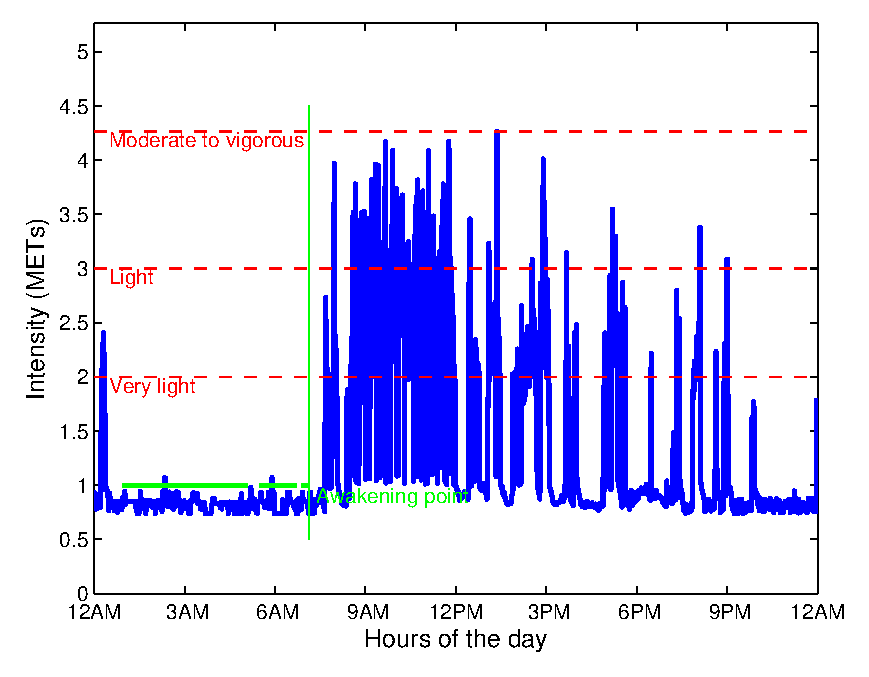
\includegraphics[width=.45\textwidth]{figure/eps/figure_1_1sub.eps}}}
%   \mbox{\subfloat[Quantization in intensity categories.]{\label{fig:1b} 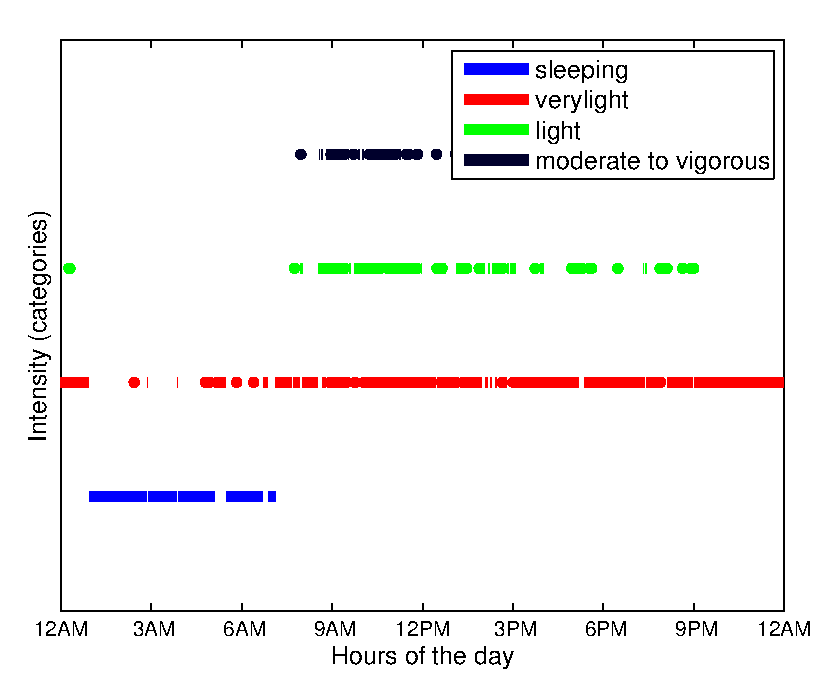
\includegraphics[width=.45\textwidth]{figure/eps/figure_2_1sub.eps}}}
%   \caption{Figure weekend-weekdays}\label{fig:1}
% \end{figure}
\begin{figure}[ht]
  \centering
  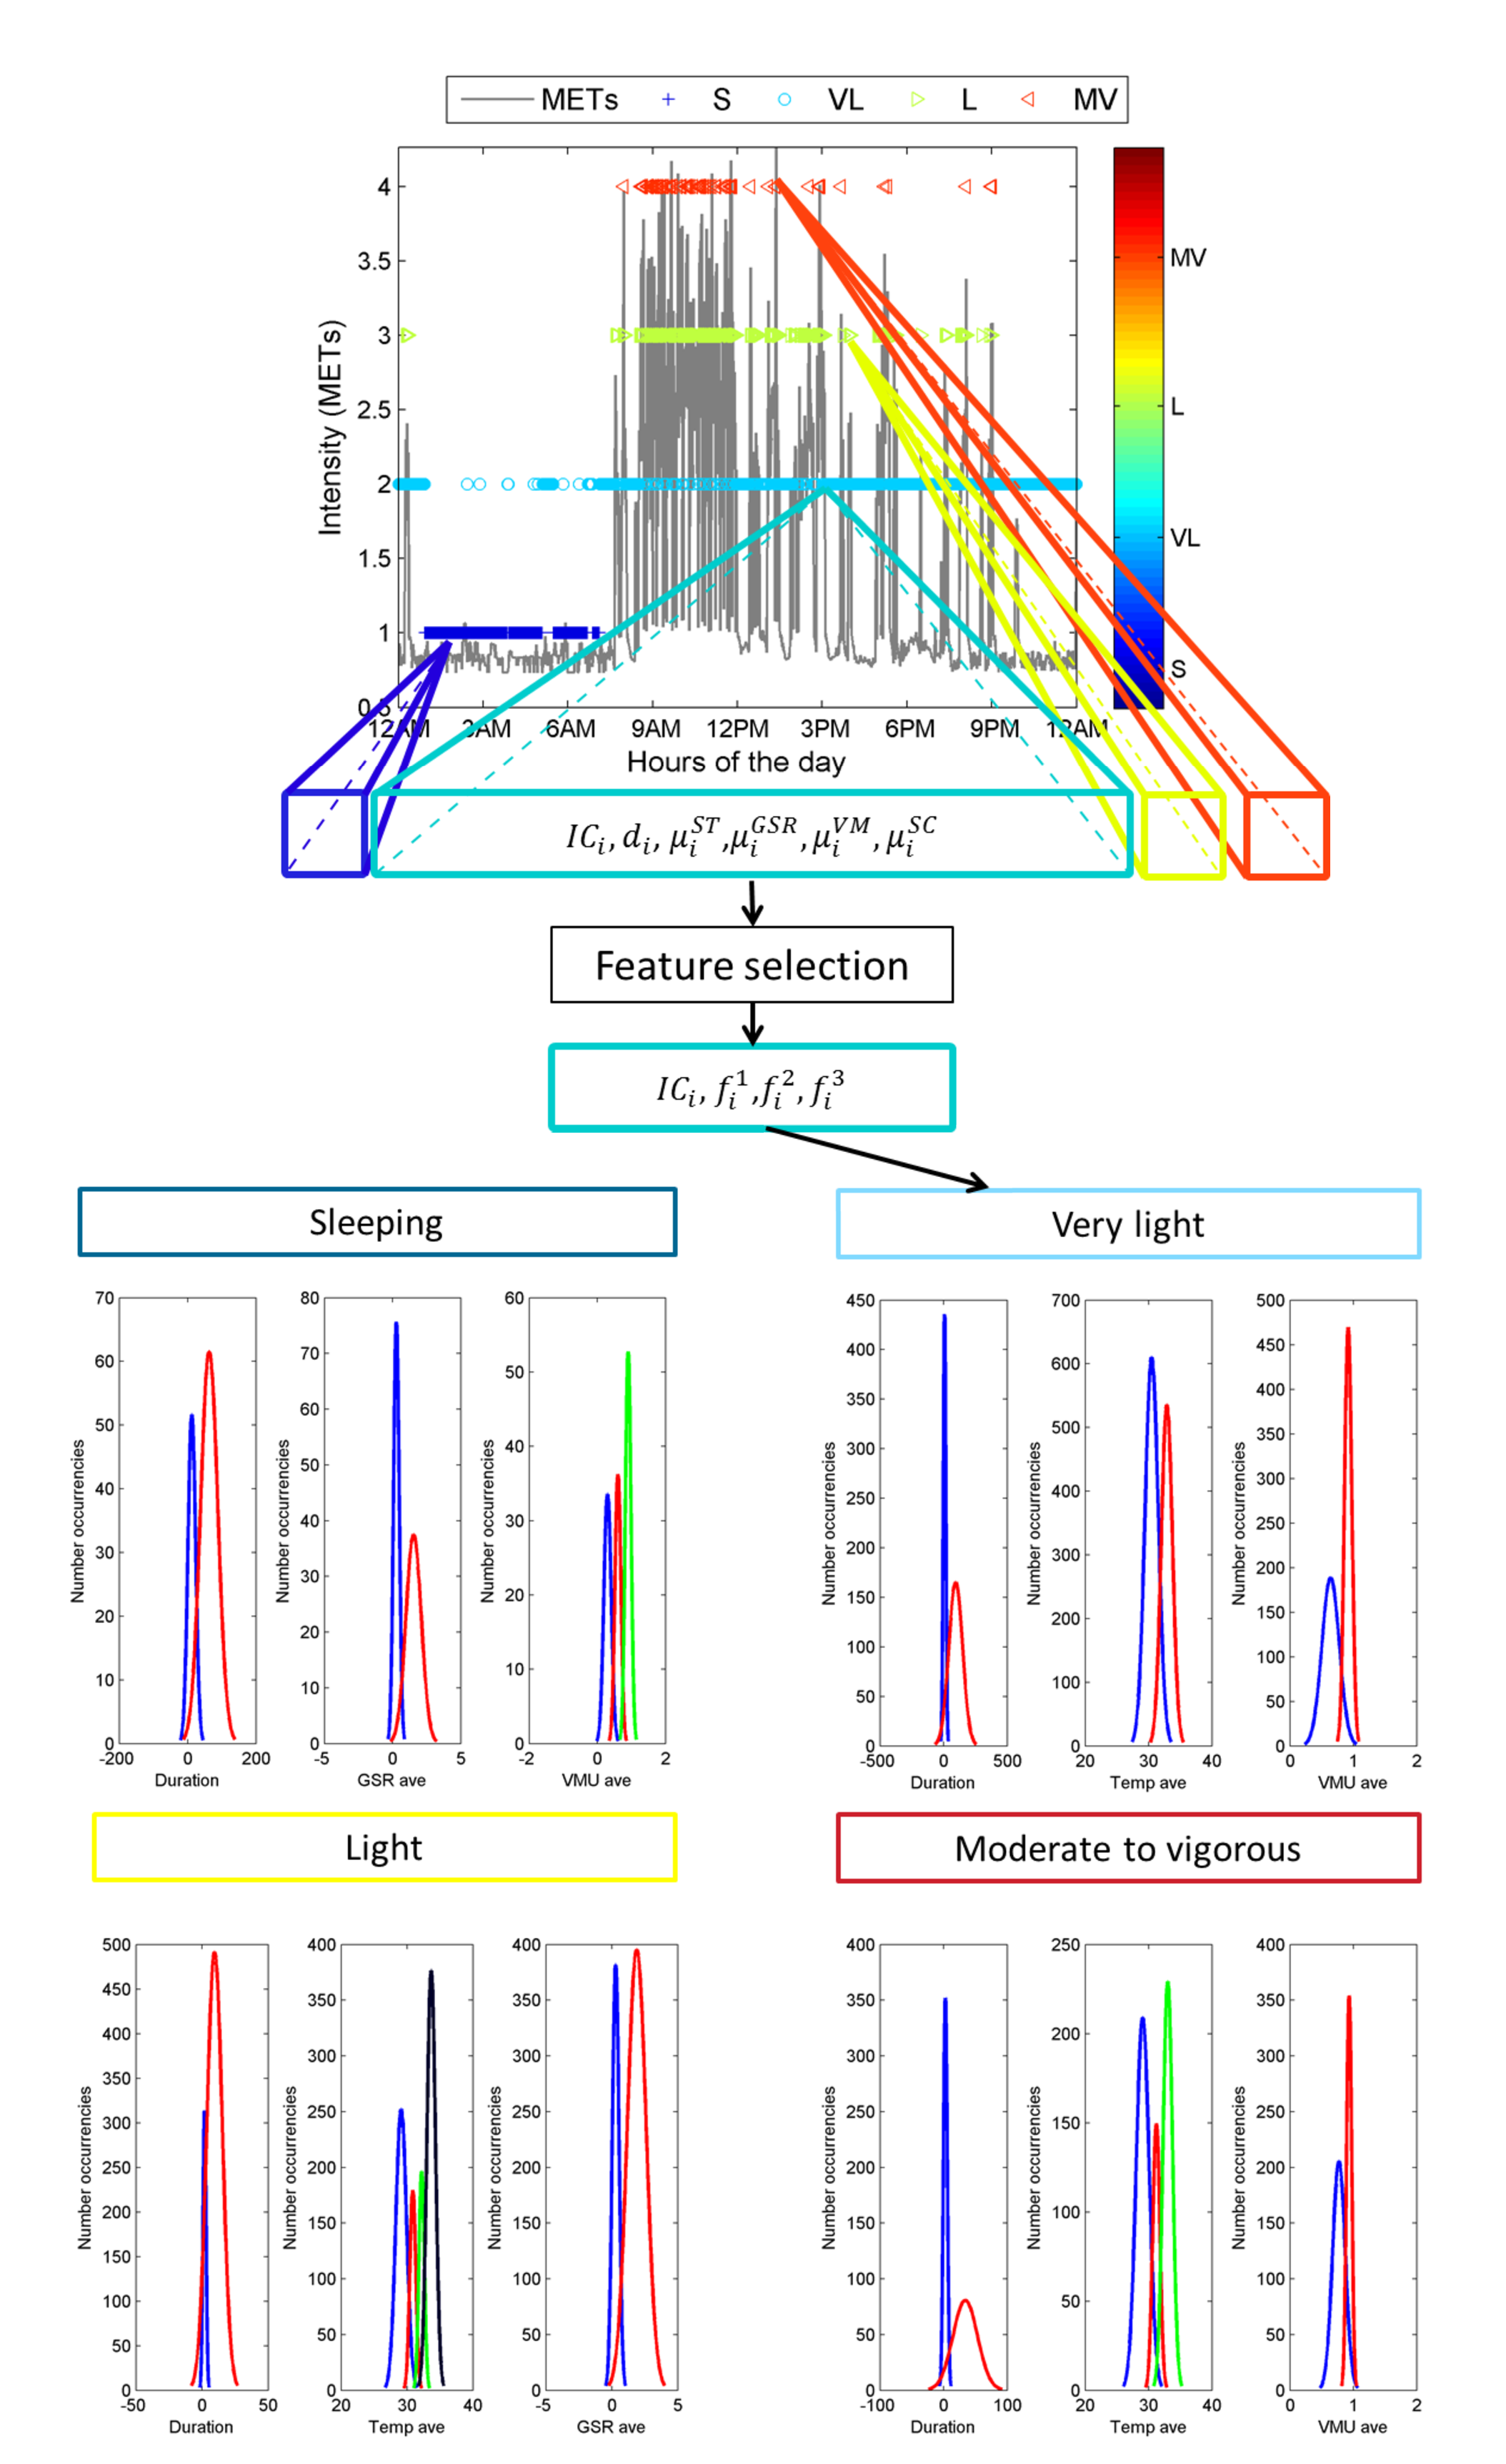
\includegraphics[width=.45\textwidth]{figure/eps/figure_11_together_mod_plus_arrow.eps}
  \caption[]{A continuous data stream representing METs value (grey line) is converted in bouts of PA intensity (blue=sleeping, ciano=verylight, green=light, and red=moderate to vigorous intensities). Features are computed within the bouts and the most relevant will be combine to create PA descriptors.}
  \label{fig:1}
\end{figure}
%%%%%%%%%%%%%%%%%%%%%%%%%%%%%%%%%%%%%%%%%%%%%%%%%%%%%%%%%%%%%%%%%%%%%%%%%%%
Consecutive minutes exhibiting the same $ICs$ are then grouped together in intensity bouts ($IB$) of variable duration ($d$). In each $IB$ we calculated the mean $\mu$ of $ST$, $GSR$, $VM$ and $SC$.
%\begin{itemize}
%\item Skin temperature ($u_{skt}$, $\sigma_{skt}$)
%\item Galvanic skin response ($u_{grs}$, $\sigma_{grs}$)
%\item Vector magnitude unit ($u_{vmu}$, $\sigma_{vmu}$)\\where $vmu=\sqrt{Acc_{x}^2+Acc_{y}^2}$ 
%\item Step counts ($u_{sc}$, $\sigma_{sc}$).
%\end{itemize}
The original sensor data stream is then represented by a series of intensity bouts where each bout is fully characterized by a 6-elements feature vector $\tilde{V}$ 
\begin{equation}
\tilde{V} = [IC, d, \mu_{ST}, \mu_{GSR}, \mu_{VM}, \mu_{SC}].
\end{equation}
Subsequently, for each intensity category ($S$, $VL$, $L$ and $VL$) the most relevant subset of features was selected such that the multi-cluster structure of the data can be best preserved. 
Features were selected using the Multi-Cluster Feature Selection (MCFS) that deploys spectral regression with \emph{l$_1$}-norm 
regularization in order to select features jointly instead of evaluating each feature independently~\cite{Cai_2010}. The feature vector $\tilde{V}$ can then be simplified according to
\begin{equation}
V = [IC, f_{1},f_{2},f_{3}].
\end{equation}
The reader might think about this step as a stemming procedure that removes redundant letters that might confuse the model.
The selected features $f_{j\in\{1,2,3\}}$ obviously might be different for each intensity and are shown in the bottom part of Fig.~\ref{fig:1}. 
\par To generate the vocabulary of words each of the selected features was first standardized and then mapped into a set of discrete levels using a K-means clustering algorithm. The algorithm automatically selects for each feature the number of levels $K^{f_{j}}$ (which could be interpreted as the letters of our words) in a way that the corresponding clustering results $L_{p\in\{1:K\}}$ are the most stable under small perturbations of the input dataset as described in~\cite{Luxburg_2010}.\\
Levels are sorted according to their mean value $\bar{L_{p}}$ in ascending order such that: first level ($L_{1}$) represents clusters with the smallest feature values and the last level ($L_{K}$) represents clusters with the highest feature values. 
Mean value and variance of the levels were stored and used to create the documents as described later in section~\ref{subsec:topicinf}. The vocabulary of terms was built by allowing all the possible combinations between levels sharing the same $IC$. 
%$N = K_{1} \cdot K_{2} \cdot K_{3}$ 
For the sleeping category, for example, the feature $f_{1}=d$, $f_{2}=\mu_{GSR}$ and $f_{3}=\mu_{VM}$ were selected and divided in $K^{f_{1}}=K^{f_{2}}=2$ and $K^{f_{3}}=3$ levels respectively.
The $N^{S}$ ($N^{S}=K^{f_{1}} \cdot K^{f_{2}} \cdot K^{f_{3}}$) terms of the vocabulary describing the sleeping intensity category ($t^{S}_{i\in\{1:N^{S}\}}$) are:
\begin{eqnarray}\label{eq:words}
t^{S}_{1}=\{L_{1}^{f_{1}}\_L_{1}^{f_{2}}\_L_{1}^{f_{3}}\}\nonumber\\
t^{S}_{2}=\{L_{1}^{f_{1}}\_L_{1}^{f_{2}}\_L_{2}^{f_{3}}\}\nonumber\\
...\nonumber\\
t^{S}_{12}=\{L_{2}^{f_{1}}\_L_{2}^{f_{2}}\_L_{3}^{f_{3}}\}\nonumber\\
\end{eqnarray}
The sum of terms across different activity levels is the total number of words.
%The feature selected for each $IC$, the $L_{p}$ levels for each feature are shown in~\ref{}. {\color{red}ADD TABLE WITH FEATURES, MEAN AND VARIANCE LEVELS.} 
In particular a total of 48 terms were created (12 for S, 8 for VL, 16 for L and 12 for MV intensity). Note that we did not need to specify the number of unique artificial words (vocabulary size) beforehand.
%Since rare words (defined as occurring less than twice in a document) do not affect much the inference process we did not consider them further in the analysis. 
As a last step frequent words (occurring at least in the 94\% of the documents) were removed because they will be placed by the model with high probability in all the topics. In other words they occur so frequently that they are more likely to obscure than facilitate a meaningful decomposition of the collection of documents. 
%{\color{red}SPECIFY WORDS THAT WERE REMOVED IN THE TABLE AND MAYBE PUT A FIGURE SHOWING THE FREQUENCY OF THE WORDS?.}

%The words used to create the set of topics are listed in table~\ref{table:Table 3}~\ref{table:Table 4}~\ref{table:Table 5}~\ref{table:Table 6}


%%%%%%%%%%%%%%%%%%%%%%%%%%%%	FIGURE FEATURE SELECTION		%%%%%%%%%%%%
%\newpage
%\begin{figure*}[ht]
%\centering
%  \mbox{\subfloat[Sleeping.]{\label{fig:5a} 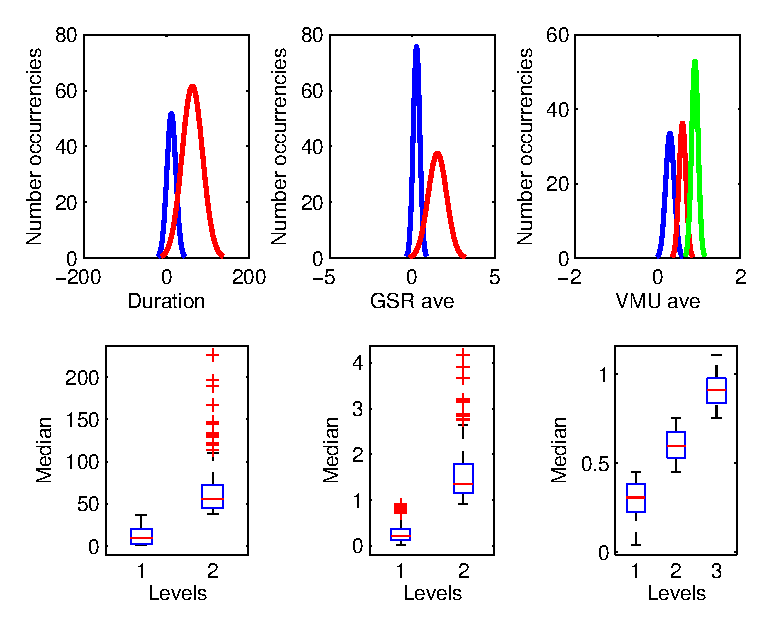
\includegraphics[width=.45\textwidth]{figure/eps/figure_5_sleeping.eps}}}
%  \mbox{\subfloat[Very light.]{\label{fig:5b} 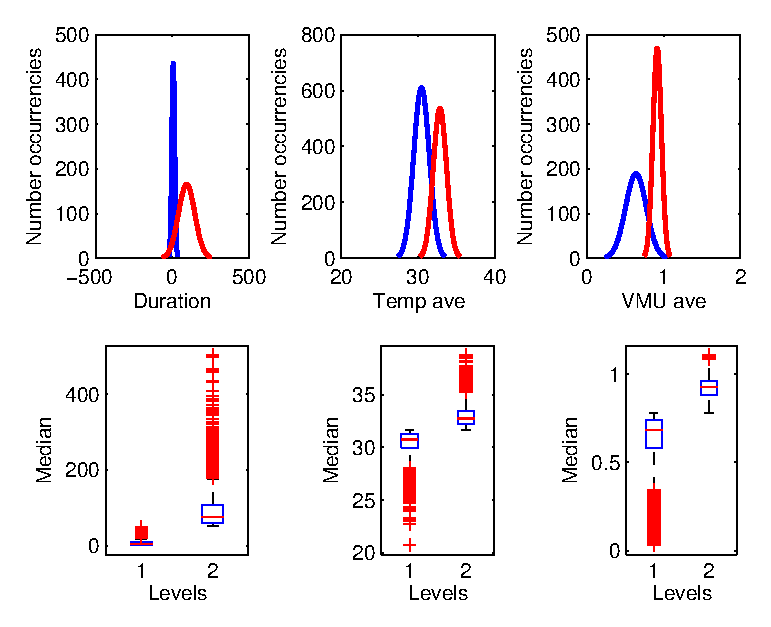
\includegraphics[width=.45\textwidth]{figure/eps/figure_5_verylight.eps}}}
%  \mbox{\subfloat[Light.]{\label{fig:5c} 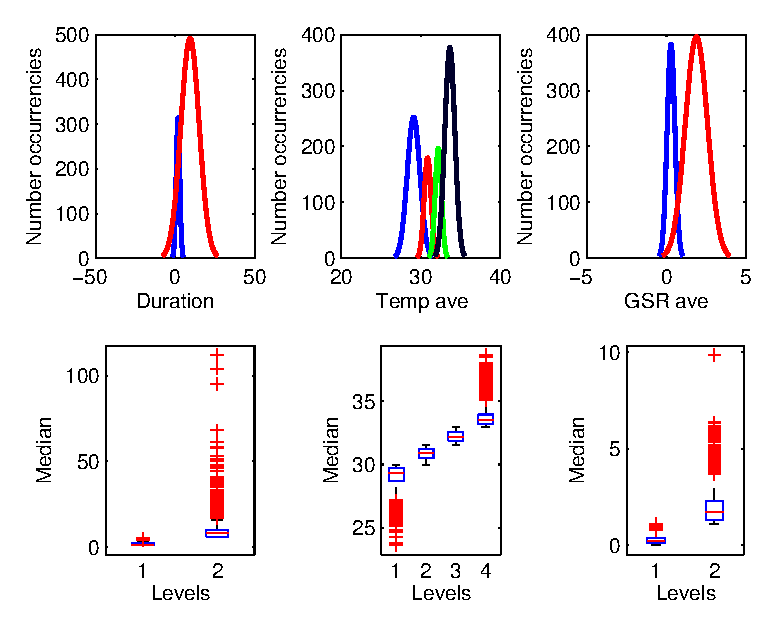
\includegraphics[width=.45\textwidth]{figure/eps/figure_5_light.eps}}}
%  \mbox{\subfloat[Moderate to vigorous.]{\label{fig:5d} 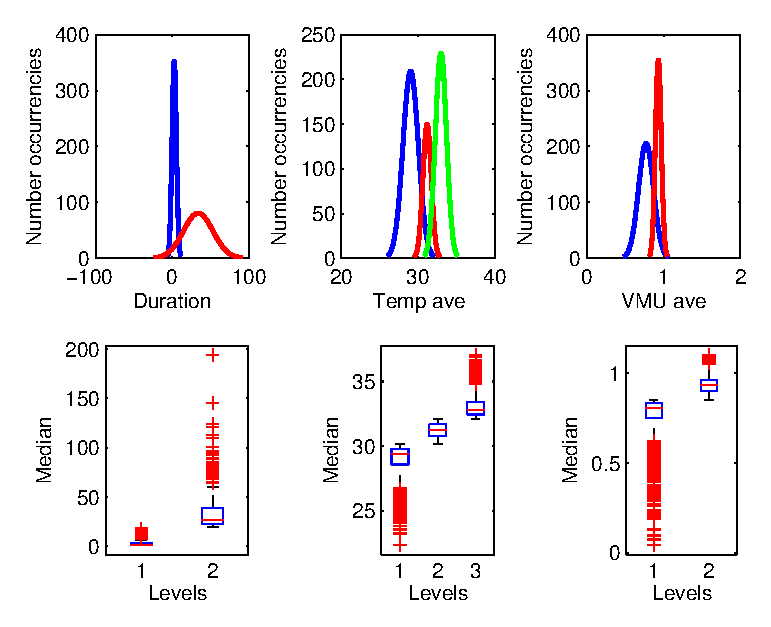
\includegraphics[width=.45\textwidth]{figure/eps/figure_5_MVPA.eps}}}
%\caption{Scatter plot selected features}\label{fig:5}
%\end{figure*}




%\newpage
%%%%%%%%%%%%%%%%%%%%%%%%%%%%	TABLE FEATURE PER CLUSTER	%%%%%%%%%%%%%%%%
%
%
%\begin{table}[H!]                                                                                             
%{\tiny
%\centering                                                                                                    
%\begin{tabular}{|c|c|c|c|c|c|c|c|c|c|}                                                                        
%\hline                                                                                                        
% & Dur & T ave & \textbf{GSR} ave & \textbf{VMU} ave & Step count ave & T std & GSR std & VMU std & \textbf{Step count std} \\
%\hline
%Word 1 & 29.69 & 33.31 & 0.39 & 0.55 & 0.40 & 0.23 & 0.03 & 0.08 & 1.31 \\
%\hline
%Word 2 & 29.30 & 33.14 & 0.28 & 0.87 & 0.00 & 0.21 & 0.01 & 0.02 & 0.01 \\
%\hline
%Word 3 & 30.48 & 33.26 & 0.27 & 0.42 & 0.00 & 0.24 & 0.01 & 0.04 & 0.01 \\
%\hline
%Word 4 & 30.87 & 33.67 & 1.54 & 0.62 & 0.00 & 0.23 & 0.06 & 0.03 & 0.02 \\
%\hline
%\end{tabular}
%\caption{Average values cluster variables after removing frequent words (sleeping)}                                                                             
%\label{table:Table 3} 
%}
%\end{table}       
%
%
%\begin{table}[H!]                                                                                             
%{\tiny
%\centering                                                                                                    
%\begin{tabular}{|c|c|c|c|c|c|c|c|c|c|}                                                                        
%\hline                                                                                                        
% & \textbf{Dur} & \textbf{T ave} & \textbf{GSR} ave & VMU ave & Step count ave & T std & GSR std & VMU std & Step count std \\
%\hline
%Word 1 & 14.20 & 32.76 & 1.75 & 0.87 & 1.86 & 0.12 & 0.06 & 0.06 & 2.69 \\
%\hline
%Word 2 & 108.00 & 32.42 & 0.34 & 0.84 & 0.84 & 0.39 & 0.04 & 0.11 & 2.74 \\
%\hline
%\end{tabular}
%\caption{Average values cluster variables after removing frequent words (very light)}                                                                            
%\label{table:Table 4}                                                                                         
%}
%\end{table}  
%
%
%\begin{table}[H!]                                                                                             
%{\tiny
%\centering                                                                                                    
%\begin{tabular}{|c|c|c|c|c|c|c|c|c|c|}                                                                        
%\hline                                                                                                        
% & \textbf{Dur} & T ave & \textbf{GSR ave} & VMU ave & Step count ave & T std & GSR std & VMU std & \textbf{Step count std} \\
%\hline
%Word 1 & 19.19 & 31.86 & 0.42 & 0.87 & 14.91 & 0.16 & 0.02 & 0.05 & 8.87 \\
%\hline
%Word 2 & 4.79 & 32.44 & 1.94 & 0.89 & 17.36 & 0.07 & 0.05 & 0.04 & 8.03 \\
%\hline
%Word 3 & 4.17 & 32.55 & 0.35 & 0.91 & 39.05 & 0.06 & 0.01 & 0.05 & 28.95 \\
%\hline
%Word 4 & 4.17 & 31.72 & 0.30 & 0.89 & 12.29 & 0.05 & 0.01 & 0.04 & 4.42 \\
%\hline
%Word 5 & 5.37 & 31.56 & 0.32 & 0.89 & 19.65 & 0.07 & 0.01 & 0.05 & 11.77 \\
%\hline
%\end{tabular}
%\caption{Average values cluster variables after removing frequent words (light)}                                                                                
%\label{table:Table 5}                                                                                         
%}
%\end{table}  
%
%
%\begin{table}[H!]                                                                                             
%\centering                                                                                                    
%{\tiny
%\begin{tabular}{|c|c|c|c|c|c|c|c|c|c|}                                                                        
%\hline                                                                                                        
% & Dur & T ave & \textbf{GSR} ave & VMU ave & \textbf{Step count ave} & \textbf{T std} & GSR std & VMU std & Step count std \\
%\hline
%Word 1 & 6.65 & 31.10 & 0.33 & 0.88 & 15.26 & 0.09 & 0.02 & 0.05 & 9.34 \\
%\hline
%Word 2 & 7.05 & 31.26 & 0.40 & 0.94 & 79.13 & 0.10 & 0.02 & 0.03 & 18.57 \\
%\hline
%Word 3 & 9.56 & 31.94 & 2.27 & 0.90 & 30.79 & 0.10 & 0.11 & 0.05 & 14.20 \\
%\hline
%Word 4 & 30.78 & 28.95 & 0.55 & 0.87 & 35.00 & 1.10 & 0.19 & 0.07 & 16.53 \\
%\hline
%\end{tabular}
%\caption{Average values cluster variables after removing frequent words (MVPA)}                                                                                 
%\label{table:Table 6}                                                                                         
%}
%\end{table}  
%
%%%%%%%%%%%%%%%%%%%%%%%%%%%%%%%%%%%%%%%%%%%%%%%%%%%%%%%%%%%%%%%%%%%%%%%%%%%%

\subsection{Topic discovery}
For topic discovery we used the LDA implementation of~\cite{Blei_2003} and we considered each day of assessment as a separate document.
%
%(1) An instance of the vocabulary was assigned to each $IB_{i}$ by associating the selected features of $V_{i}$ with their closest levels and then concatenating the 3 closest levels found.
%
Each $IB$ was mapped with an instance of the vocabulary by associating the selected features in $V$ with their closest levels and then concatenating the 3 closest levels found. 
%
%(3) For each $IC$ we assigned a discrete term of the vocabulary that minimizes the distances between the selected features and the levels. 
The distance for each bout between the feature point $f_{j}$  and all the levels $L_{p}$ are
%\begin{equation}\label{eq:distance}
%d_{i,p}({f^{j},L_{p}}) = \mid{f^{j}_{i}-\tilde{L}^{f^{j}}_{p}}\mid , \forall p=\{1,...,K^{f^{j}}\}.
%\end{equation}
\begin{equation}\label{eq:distance}
d_{p}({f_{j},L_{p}}) = \frac{\left|f_{j}-\bar{L}^{f_{j}}_{p}\right|}{\sigma_{p}} , \forall p=\{1,...,K^{f^{j}}\}.
\end{equation}
Once that a term of the vocabulary was assigned to each $IB$, documents were created constructing for each day a histogram of terms occurrences. 
We chose the number of topics ($T$) equal to 18 and set the hyperparameter $\alpha$ equal to 0.01 as in~\cite{Huynh_2008}. Hyperparameters are optimized iteratively
within a variational expectation maximization (EM) algorithm based on observed words from 18 randomly selected documents (6 healthy subjects, 6 COPD patients).
%The discovered topics are ordered within a document according to their variational posterior Dirichlets. Topics are presented as
%distributions over the vocabulary.
%\begin{equation}
%\log{p(w | z=k)}.
%\end{equation} 
%To evaluate the topic model we used the LDA implementation
%of [1], which includes an iterative optimization for topic
%model parameters ;  regarding model likelihood. The initial
%hyperparameter  was set to  = 0:01 as suggested by
%[4].

\subsection{Topic inference}\label{subsec:topicinf}
Once the topics are calculated, to know which one was active during the different parts of the day, we inferred documents composed by day segments. Differently from the documents used to discover the topics, each document represents a mixture of terms over a window of time $D$. We used sliding windows of 30 minutes as suggested in~\cite{Seiter_2014}. 
%We used sliding windows of 30 minutes with 90\% overlap as suggested in~\cite{Seiter_2014}. 
For each window we constructed a histogram of terms occurrences by mapping the bouts in $D$ to the words in the vocabulary giving soft assignments. For each feature point in $V$ we calculated the distances $d_{1...K^{f_{j}}}({f_{j},L_{p}})$ from the mean values of associated levels as in~(\ref{eq:distance}).
The distances were converted in weights according to
%\begin{eqnarray}
%w_{i,p}(f^{j},L_{p})=\frac{e^{-\frac{d_{i,p}}{\sigma_{p}}}}{\sum_{p=1}^{K^{f^{j}}} e^{-\frac{d_{i,p}}{\sigma_{p}}}}
%\end{eqnarray}
\begin{eqnarray}
w_{p}(f_{j},L_{p})=\frac{e^{-d_{p}}}{\sum_{p=1}^{K^{f_{j}}} e^{-d_{p}}}
\end{eqnarray}
Thus smaller distances imply higher weights and the weights for different levels of one selected feature sum up to one. 
%The parameter $\sigma$ controls how fast the weights decline for more distant clusters.
%or use the mahalanobis distance instead
We then concatenate the weights as we did in~(\ref{eq:words}) creating combination of weights, each of one assigned to the related term of the vocabulary. 
Summing up the weights of a specific term across the feature selected and dividing by the sum of the weights of all the terms we get values comprised between 0 and 1 that indicate the probability that the term appear in the document segment $D$. Weights of terms referring to other intensities will be set to 0.
Recalling the example with a sleeping bout we have 12 weights $G_{i}^{S}$
\begin{eqnarray}
G^{S}_{1}=\frac{w_{1}^{f_{1}}+w_{1}^{f_{2}}+w_{1}^{f_{3}}}{\sum{_{t=1}^{N^{S}}}G_{t}}\nonumber\\
%\{w_{i,1}^{f_{1}}\_w_{i,1}^{f_{2}}\_w_{i,1}^{f_{3}}\}\nonumber\\
...\nonumber\\
G^{S}_{2}=\frac{w_{1}^{f_{1}}+w_{1}^{f_{2}}+w_{2}^{f_{3}}}{\sum{_{t=1}^{N^{S}}}G_{t}}\nonumber\\
%w^{S}_{2}=\{w_{i,1}^{f_{1}}\_w_{i,1}^{f_{2}}\_w_{i,2}^{f_{3}}\}\nonumber\\
...\nonumber\\
G^{S}_{12}=\frac{w_{2}^{f_{1}}+w_{2}^{f_{2}}+w_{3}^{f_{3}}}{\sum{_{t=1}^{N^{S}}}G_{t}}\nonumber\\
%w^{S}_{12}=\{w_{i,2}^{f_{1}}\_w_{i,2}^{f_{2}}\_w_{i,3}^{f_{3}}\}\nonumber\\
\end{eqnarray}
We next use the weights associated to each term to construct documents of size $D$. More specifically, for each term we sum up the weights $W_{t}$ over a feature window of length $D$, and then generate $m_{W_{t}}$ instances of the term by multiplying the sum of this weights by the document length $D$ and rounding to the next integer. 


%\newpage
%\input{results_fix_94_18.tex}
\section{Qualitative analysis}
Since PA measures during the weekdays and the weekend days are known to be different \cite{Watz_2009}, results were computed separately and only the ones relative to weekdays will be presented.
Figure~\ref{fig:10} illustrates the distribution of the dicovered routines $\beta_{1,..,18}$ over the terms of the vocabulary.
%% BETAS (DISTRIBUTION OVER THE WORDS)
\begin{figure}[ht!]
  \centering
  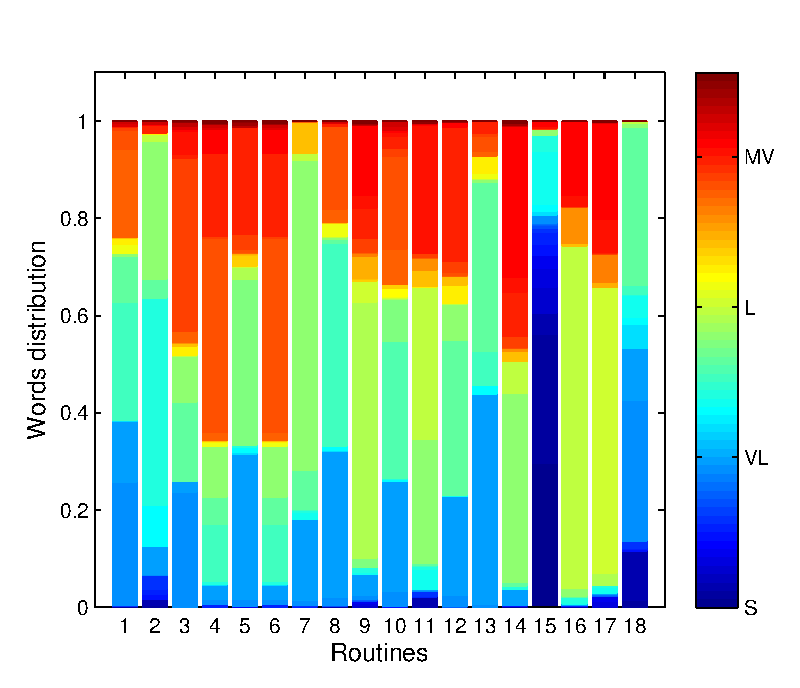
\includegraphics[width=.45\textwidth]{figure/eps/figure_10.eps}
  \caption[]{Distribution over the words}
  \label{fig:10}
\end{figure}
Four routines ($R2$, $R7$, $R13$, $R18$) related to low intensity levels, seven routines ($R4$, $R6$, $R9$, $R11$, $R14$, $R16$, $R17$) related high intensity levels and six routines ($R1$, $R3$, $R5$, $R8$, $R10$, $R12$) composed by a combination of VL, L and MV descriptors were discovered in data from 66 COPD patients and 66 healthy subjects. A separate routine ($R15$) characterizing the sleeping behavior was also found.
Each of these routines is characterized by a combination of words that in turn varies in relation to the feature levels. A detailed description of the routines with the 3 most important descriptors associated can be found in table~\ref{table:routines}. The words composing a particular routine are listed together with their occurrence probability (e.g. the first word of $R1$: \textit{[2 1 1 1]} refers to the descriptor \textit{$VL\_1^{d}\_1^{ST}\_1^{VM}$} and has an associated probability equal to 25\% ). Higher the probability, higher the importance of the descriptor for the routine.
%%%%%%%%%%%%%%%%%%%%%%%%%%%%%	TABLE RoutineS DISCOVERED	%%%%%%%%%%%%%%%%%%%%
%\newpage
%\begin{sidewaystable*}[H!]
%\centering
%\begin{tabular}{|c|c|c|c|c|c|c|c|c|c|c|c|c|c|c|c|c|c|c|c|}
%\hline
%Topic1  &    &  Topic2  &   &  Topic3  &    &  Topic4  &   & Topic5  &    &  Topic6  &    &  Topic7  &    &  Topic8  &    &  Topic9  &    &  Topic10  &	\\
%\hline
%\hline
%3 1 1 1  &  0.1  &  3 1 2 5  &  0.1  &  4 2 2 1  &  0.2  &  3 1 2 4  &  0.1  &  3 1 1 1  &  0.3  &  2 2 1 1  &  0.2  &  4 2 1 1  &  0.1  &  1 1 3 1  &  0.2  &  4 3 2 1  &  0.1  &  3 2 2 1  &  0.2  \\
%\hline
%4 1 2 1  &  0.1  &  4 1 2 1  &  0.1  &  3 1 2 4  &  0.1  &  2 2 2 1  &  0.1  &  3 1 1 4  &  0.1  &  1 1 2 1  &  0.2  &  3 1 1 1  &  0.1  &  2 1 1 2  &  0.1  &  2 1 2 3  &  0.1  &  3 2 1 1  &  0.1  \\
%\hline
%4 1 1 1  &  0.1  &  3 1 2 6  &  0.1  &  3 1 2 5  &  0.1  &  3 1 2 3  &  0.1  &  3 1 1 5  &  0.1  &  2 2 2 1  &  0.1  &  4 3 1 1  &  0.1  &  1 1 3 2  &  0.1  &  3 1 2 4  &  0.1  &  4 3 2 1  &  0.1  \\
%\hline
%2 1 2 3  &  0.1  &  2 1 2 5  &  0.1  &  2 1 2 4  &  0.1  &  3 1 2 2  &  0.1  &  2 1 2 4  &  0.0  &  2 1 1 2  &  0.1  &  2 1 1 6  &  0.0  &  3 1 1 1  &  0.1  &  3 1 2 3  &  0.1  &  3 2 2 3  &  0.0  \\
%\hline
%3 1 2 3  &  0.1  &  3 1 2 4  &  0.1  &  3 1 2 3  &  0.1  &  4 2 2 1  &  0.1  &  3 1 1 3  &  0.0  &  1 1 1 1  &  0.1  &  3 1 1 6  &  0.0  &  2 2 2 1  &  0.1  &  3 1 2 5  &  0.1  &  3 2 2 4  &  0.0  \\
%\hline
%3 1 2 2  &  0.0  &  2 1 2 6  &  0.1  &  2 1 2 3  &  0.1  &  4 2 2 3  &  0.0  &  3 1 1 6  &  0.0  &  1 1 2 2  &  0.0  &  3 1 1 7  &  0.0  &  1 2 3 1  &  0.0  &  3 1 2 2  &  0.1  &  2 1 2 3  &  0.0  \\
%\hline
%2 1 2 2  &  0.0  &  4 1 2 5  &  0.0  &  4 2 2 5  &  0.0  &  2 1 2 4  &  0.0  &  2 1 1 4  &  0.0  &  1 1 1 2  &  0.0  &  3 1 1 5  &  0.0  &  3 1 2 4  &  0.0  &  2 1 2 4  &  0.0  &  3 2 2 5  &  0.0  \\
%\hline
%3 1 1 4  &  0.0  &  3 1 2 7  &  0.0  &  3 1 2 6  &  0.0  &  4 2 2 2  &  0.0  &  3 1 2 4  &  0.0  &  3 1 1 6  &  0.0  &  4 1 1 1  &  0.0  &  2 1 2 2  &  0.0  &  2 1 2 2  &  0.0  &  2 1 2 4  &  0.0  \\
%\hline
%2 1 2 4  &  0.0  &  4 1 2 6  &  0.0  &  4 2 2 4  &  0.0  &  3 1 2 5  &  0.0  &  3 1 2 5  &  0.0  &  3 1 1 5  &  0.0  &  3 1 1 3  &  0.0  &  2 2 1 1  &  0.0  &  3 1 2 6  &  0.0  &  4 2 2 1  &  0.0  \\
%\hline
%3 1 2 4  &  0.0  &  3 1 2 3  &  0.0  &  2 1 2 2  &  0.0  &  2 1 2 3  &  0.0  &  2 1 1 5  &  0.0  &  1 2 2 1  &  0.0  &  2 1 2 6  &  0.0  &  3 1 2 5  &  0.0  &  4 3 2 5  &  0.0  &  3 2 2 2  &  0.0  \\
%\hline
%3 1 1 3  &  0.0  &  4 1 2 4  &  0.0  &  3 1 1 1  &  0.0  &  2 2 1 1  &  0.0  &  2 2 1 1  &  0.0  &  3 1 1 7  &  0.0  &  4 2 2 1  &  0.0  &  1 1 2 1  &  0.0  &  4 3 2 4  &  0.0  &  2 1 2 2  &  0.0  \\
%\hline
%4 1 2 4  &  0.0  &  2 2 2 1  &  0.0  &  3 1 2 2  &  0.0  &  4 1 2 1  &  0.0  &  2 1 2 3  &  0.0  &  2 1 2 2  &  0.0  &  3 1 1 4  &  0.0  &  3 1 2 6  &  0.0  &  3 1 1 1  &  0.0  &  3 2 1 4  &  0.0  \\
%\hline
%3 1 1 5  &  0.0  &  3 1 1 6  &  0.0  &  4 2 2 6  &  0.0  &  4 2 2 4  &  0.0  &  2 1 2 5  &  0.0  &  3 1 2 6  &  0.0  &  4 2 1 7  &  0.0  &  3 1 2 3  &  0.0  &  2 1 2 5  &  0.0  &  3 2 2 6  &  0.0  \\
%\hline
%3 1 1 2  &  0.0  &  3 1 1 1  &  0.0  &  2 1 2 5  &  0.0  &  4 3 2 2  &  0.0  &  2 1 1 3  &  0.0  &  3 1 1 1  &  0.0  &  4 2 1 6  &  0.0  &  3 1 1 4  &  0.0  &  3 1 2 7  &  0.0  &  3 2 1 5  &  0.0  \\
%\hline
%4 1 2 3  &  0.0  &  2 1 2 4  &  0.0  &  4 2 2 3  &  0.0  &  4 3 2 3  &  0.0  &  3 1 2 3  &  0.0  &  1 2 1 1  &  0.0  &  3 1 1 2  &  0.0  &  3 1 1 6  &  0.0  &  4 3 2 3  &  0.0  &  3 2 1 3  &  0.0  \\
%\hline
%\end{tabular}
%\caption{Topics words-probabilities (04 002 means the second word of intensity 4}
%\label{table:Table 7}
%\end{sidewaystable*}

\begin{table}[ht!]
\centering
\scalebox{0.65}{
\begin{tabular}{|c|c|c|c|c|c|c|c|c|c|c|c|}
\hline
R1  & \%   &  R2  & \%  &  R3  &  \%  &  R4  &  \% & R5  &   \%  & R6  &   \% \\
\hline
\hline
2 1 1 1  &  0.25  &  2 2 2 2  &  0.43  &  4 1 2 1  &  0.36  &  4 1 1 2  &  0.40  &  3 1 2 2  &  0.34  &  4 1 1 2  &  0.40  \\
\hline
3 1 1 1  &  0.24  &  3 1 3 1  &  0.28  &  2 1 1 1  &  0.24  &  4 1 2 2  &  0.17  &  2 1 1 2  &  0.30  &  4 1 2 2  &  0.17  \\
\hline
4 1 1 1  &  0.18  &  2 2 1 2  &  0.09  &  3 1 2 1  &  0.16  &  3 1 1 1  &  0.12  &  4 1 2 2  &  0.22  &  3 1 1 1  &  0.12  \\
\hline
\hline
R7  &  \% &  R8  &  \%  &  R9  & \%  & R10  &  \%  & R11  &  \%  & R12  &   \% \\
\hline
\hline
3 1 3 1  &  0.64  &  3 1 1 1  &  0.42  &  3 1 3 2  &  0.53  &  3 1 1 2  &  0.28  &  3 1 4 1  &  0.31  &  3 1 2 1  &  0.32  \\
\hline
2 1 1 2  &  0.17  &  2 1 1 2  &  0.30  &  4 1 3 2  &  0.15  &  2 1 1 2  &  0.23  &  4 1 3 1  &  0.26  &  4 1 2 2  &  0.28  \\
\hline
3 1 2 1  &  0.08  &  4 1 1 2  &  0.17  &  4 1 2 2  &  0.06  &  4 1 1 2  &  0.19  &  3 1 3 1  &  0.25  &  2 1 1 2  &  0.20  \\
\hline
\hline
R13  &  \% &  R14  &  \%  &  R15  & \%  & R16  &  \%  & R17  &  \%  & R18  &   \% \\
\hline
\hline
2 1 1 2  &  0.43  &  3 1 3 1  &  0.39  &  1 1 1 1  &  0.30  &  3 1 4 1  &  0.70  &  3 1 4 2  &  0.59  &  3 1 2 1  &  0.32  \\
\hline
3 1 2 1  &  0.35  &  4 1 3 2  &  0.31  &  1 1 1 2  &  0.27  &  4 1 3 2  &  0.15  &  4 1 3 2  &  0.20  &  2 1 1 1  &  0.29  \\
\hline
3 1 1 1  &  0.07  &  4 1 2 2  &  0.09  &  2 2 2 1  &  0.11  &  3 2 4 1  &  0.07  &  4 1 3 1  &  0.07  &  2 1 1 2  &  0.11  \\
\hline
\end{tabular}
}
\caption{Routines matrix}\label{table:routines}
\end{table}
%
Figure~\ref{fig:12} illustrates the activation probability of the extracted routines when day segments of 30 minutes are sequentially inferred. The top plot and the bottom plot show respectively the routine patterns for a COPD patient and a healthy subject. It can be seen that 3 PA routines ($R2$, $R3$ and $R15$) pervade the day of a COPD patient~(top plot of Fig.~\ref{fig:12}). In particular this patient spent most of his time performing activities that involve a VL intensity descriptor of long duration, with high $\mu_{ST}$ and high $\mu_{VM}$ and a L intensity descriptor of short duration, with high $\mu_{ST}$ and low $\mu_{GSR}$. After 5 hours from the patient awakening we can see that $R13$ becomes dominant for 1 hour. This routine includes a VL descriptor of short duration, small $\mu_{ST}$ and high $\mu_{VM}$, and a L intensity descriptor of short duration, medium-low $\mu_{ST}$ and low $\mu_{GSR}$. It can also be seen that around 12 hours after the awakening of the subject $R12$ starts decreasing and $R15$, characterizing the sleeping behavior, starts to become the most active routine. On the other hand the day of a healthy subject shows a more variety of active routine patters. It can be seen from the bottom plot of Fig.~\ref{fig:12} that in the first phase of the day an alternating sequence of the routines $R13$ and $R12$ is present. $R12$ in particular is composed by descriptors related to L and MV intensities of short duration, medium-low $\mu_{ST}$ and low $\mu_{GSR}$. Around 5 hours after his awakening and in the evening before sleeping this subject assumes a similar behavior if compared to his COPD match. In particular, first routine $R12$ becomes the dominant routine for about 1 hour, and then it is active permanently until the sleeping time.
%
%
%
%
\begin{figure*}[ht]
  \centering
  \mbox{\subfloat{\label{fig:12a} 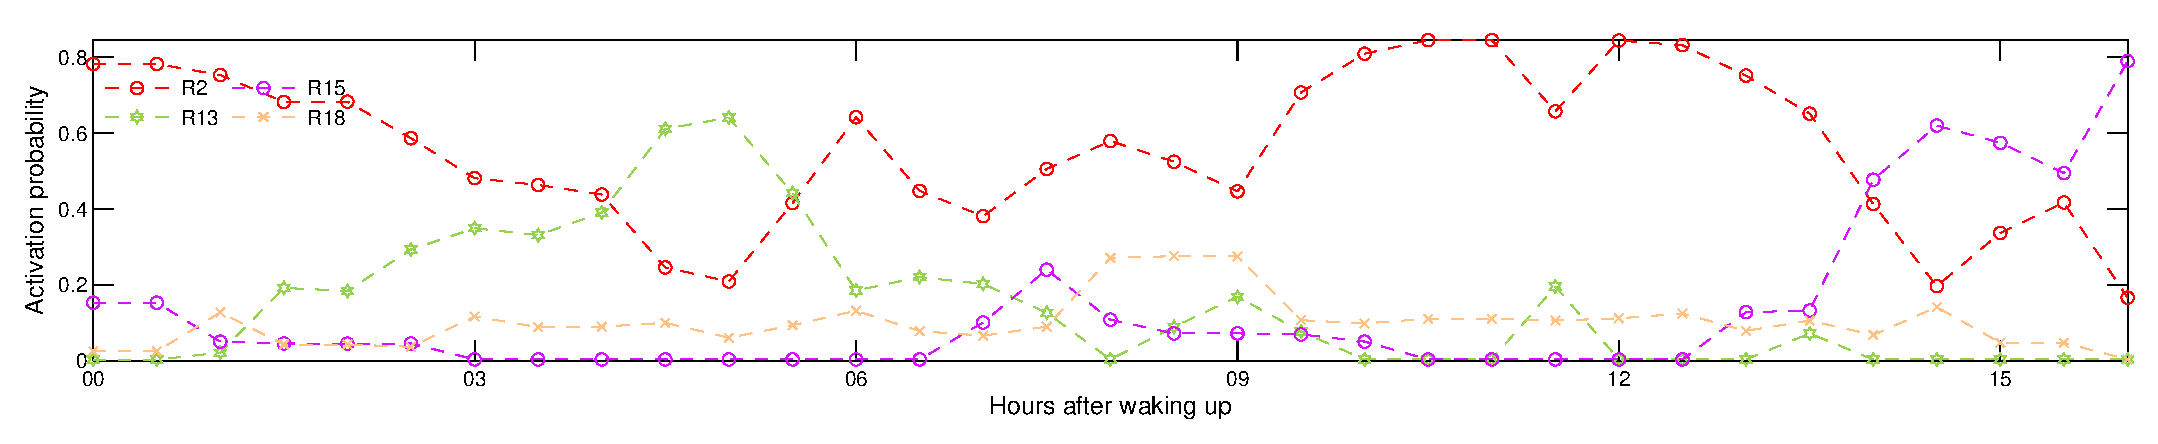
\includegraphics[width=.9\textwidth, height=3cm]{figure/eps/figure_4_1_copd_weekday.eps}}}
  \mbox{\subfloat{\label{fig:12b} 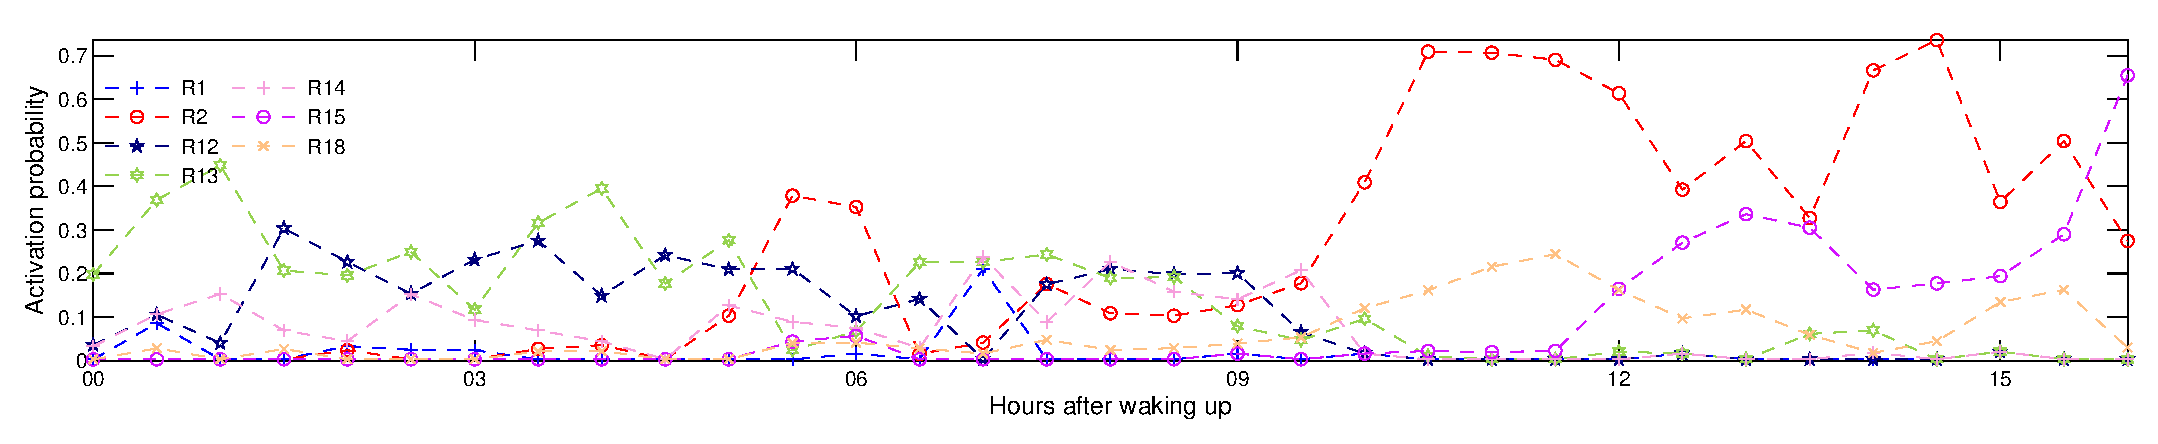
\includegraphics[width=.9\textwidth, height=3cm]{figure/eps/figure_4_1_healthy_weekday.eps}}}
  \caption{Routines found inferring a COPD patient day (top) and a healthy subject (bottom). Only topics reaching an activation $>0.2$ are shown.}\label{fig:12}
\end{figure*}
%
%
The  validity and robustness of the routines estimated are qualitatively highlighted in Fig.~\ref{fig:6}. Indeed, the routines discovered on a sub-sample of 66 patients were also inferred in the same way on data from 977 patients showing similar patterns. We can see that, on average, for COPD patients the PA descriptor $R2$ is almost always active across the days. This is consistent with other studies showing physical inactivity in patients with COPD~\cite{Troosters_2010}.
\begin{figure*}[ht]
  \centering
  \mbox{\subfloat[66 COPD patients.]{\label{fig:6a} 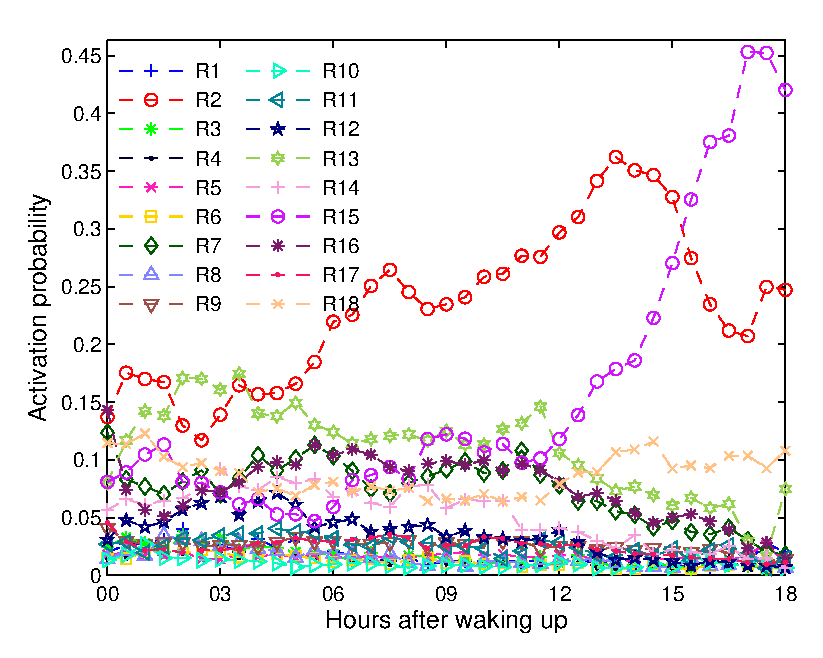
\includegraphics[width=.45\textwidth]{figure/eps/figure_4_copd_weekday.eps}}}
  \mbox{\subfloat[977 COPD patients.]{\label{fig:6b} 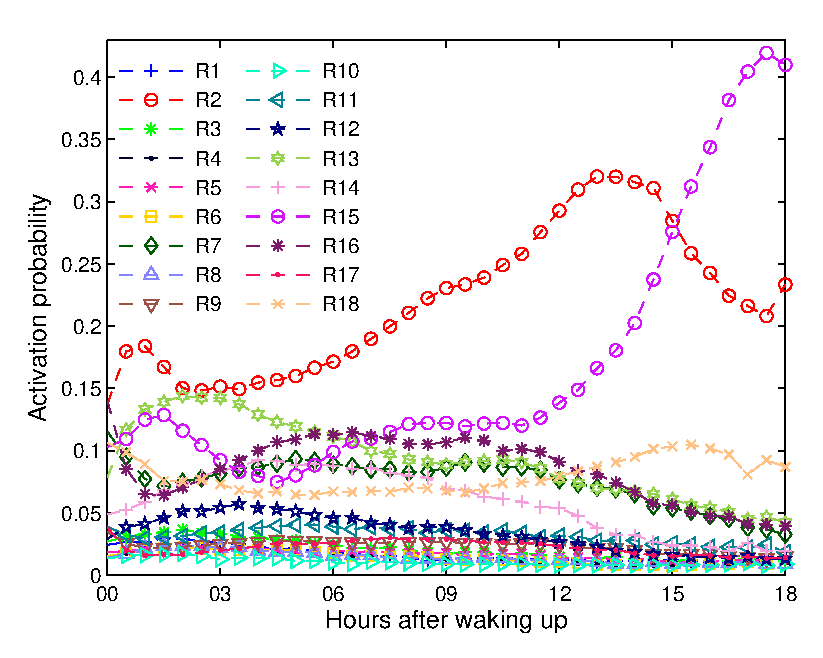
\includegraphics[width=.45\textwidth]{figure/eps/figure_4_patients_weekday.eps}}}
    \caption{Routines found inferring days from 66 COPD patients (left) and a 977 COPD patients (right). The figures show the average activation probability across the patients samples.}\label{fig:6}
\end{figure*}
%
%
Fig.~\ref{fig:7_mean} shows the average values of the routines' activation probabilities when the inference is performed on the first 6 hours after the subjects awakenings. Subjects were stratified according to their disease severity where GOLD1 and GOLD4 indicates respectively the least and most severe stage of COPD. Each point identifies the mean across all the subjects belonging to one of the 4 categories. Healthy subjects formed a separated category. 
We can observe that routines are organized according to COPD severity. In particular we can observe 4 main trends. $R2$ and $R15$ are increasing with the increase of COPD severity. In particular $R2$ represents a medium-inactive PA routine composed for the 43\% by $VL\_2^{d}\_2^{ST}\_2^{VM}$ and for the 28\% by $L\_1^{d}\_3^{ST}\_1^{GSR}$. The first PA descriptor represents very light intensity movements that cause a moderate increase of the temperature and that last for a long duration. The second descriptor represent light intensity movements characterized by short duration and a high physiological response (high body temperature). The positive trend is interrupted in the most severe group of patients that compensate a smaller value for $R2$ with a higher value of $R16$. This PA routine is characterized from PA descriptors including $L$ and $MV$ intensities and characterized by higher physiological responses if compared to $R2$. This might indicate a bigger effort in performing activities.
Another positive trend is shown by $R15$ representing the time spent while performing a very inactive behavior (mainly sleeping).
On the other hand we can note that $R13$, $R12$ and $R1$ decrease with an increase in COPD severity. These 3 routines indicate movements performed with medium ($R13$) and high ($R1$ and $R12$) activity intensities characterized by small physiological responses.
%
\begin{figure}[ht]
  \centering
%  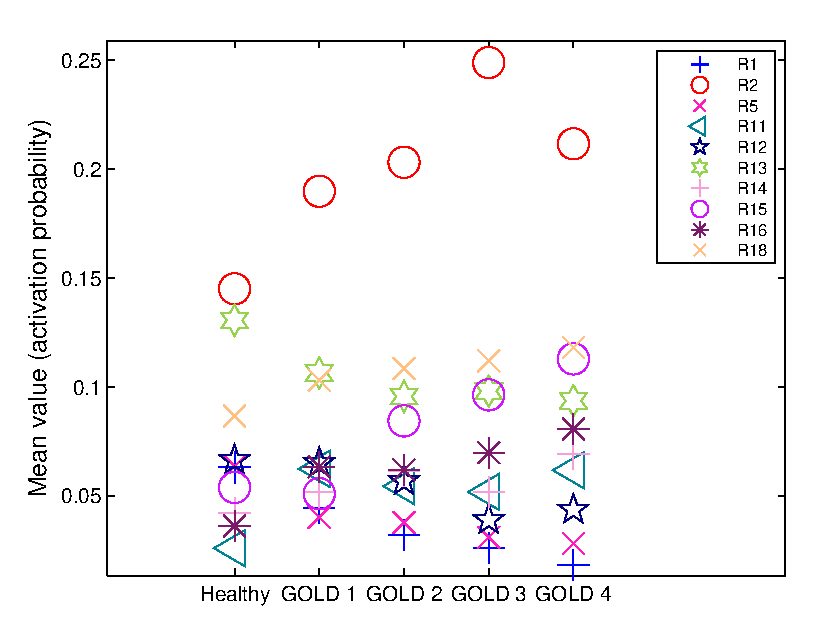
\includegraphics[width=.45\textwidth]{figure/eps/figure_7_trend_all_weekday.eps}
  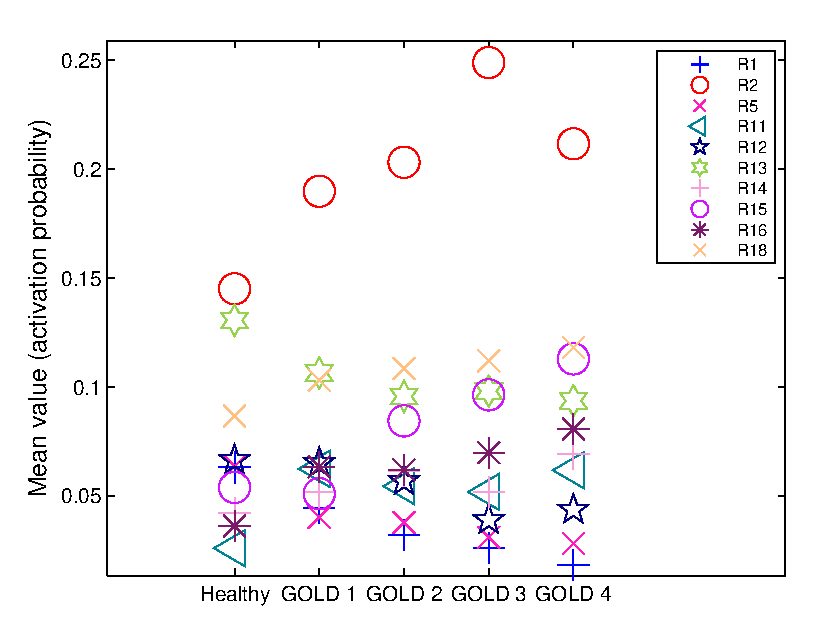
\includegraphics[width=.45\textwidth]{figure/eps/figure_7_trend_all_weekday.eps}
  \caption[]{Activation topic averages after stratification for COPD severity across 6h weekday. Inference was performed in the first 6 hours after the awakenings from the night sleep.}
  \label{fig:7_mean}
\end{figure}
Of particular interest are $R1$ and $R13$ since they are weakly but significantly correlated with $FEV_{1},\%predicted$ ($\rho=0.2$, $p=4e^{-10}$ and $\rho=1.8$, $p=1.84e^{-8}$ respectively). No correlation was found with BMI and age for $R1$. $R13$ is weakly correlated with age ($\rho=-0.18$, $p=5.3e^{-9}$). Differently from other results in literature where PA measures were highly correlated with BMI, the routines discovered seems to be decoupled from it and, although a more detailed analysis is necessary, they seem reflecting the stage of the disease as measured by common clinical practice.
In more, performing ANOVA test statistical differences have been found in the percentage of activation of $R1$ between GOLD1, GOLD3 and GOLD4 and between GOLD2 and GOLD4. Regarding $R13$ statistical differences have been found between GOLD1, GOLD3 and GOLD4, and between GOLD2, GOLD3 and GOLD4.



%\newpage
%\section{Discussion}


\section{Conclusion}
Unsupervised discovery of latent structures in data from activity sensors is becoming of increased relevance 
due to the increasing amount of available activity data.
The paper contributes to this field in different ways. First of all, real-life data 
is used concerning a relatively large population involving healthy and COPD patients. 
Secondly, the design and usage of tools differs in a number of ways from that reported so far.
Using relatively simple assumptions and settings, it is shown that interpretable and consistent results can be obtained using the 
large set of real-life data. As such it is a encouraging step into the direction of practical applications of these techniques in daily life.




%% use section* for acknowledgement
%\section*{Acknowledgment}





% Can use something like this to put references on a page
% by themselves when using endfloat and the captionsoff option.
\ifCLASSOPTIONcaptionsoff
  \newpage
\fi



\bibliographystyle{plain}
%% argument is your BibTeX string definitions and bibliography database(s)
\small{
\bibliography{mybibfile}
}
% that's all folks
\end{document}